\documentclass[11pt]{beamer}

% 使用 ctex 宏包支持中文
\usepackage[UTF8]{ctex}
\usepackage{circuitikz}
% 设置主题颜色为清华紫
\definecolor{TsinghuaPurple}{RGB}{79, 0, 128}
\setbeamercolor{structure}{fg=TsinghuaPurple}

% 设置页面背景为白色
\setbeamercolor{background canvas}{bg=white}
\usepackage{pgfplots}
% 主题设置
\usecolortheme{default}
\useinnertheme{rounded}
\useoutertheme{infolines}

% 其他常用宏包
\usepackage{graphicx} % 插入图片
\usepackage{booktabs} % 表格
\usepackage{amssymb,amsmath} % 数学符号
\usepackage{mathrsfs} % 数学花体字母
\usepackage{hyperref} % 超链接

% 修改目录样式,去掉圆圈
\setbeamertemplate{section in toc}{\inserttocsection}
\setbeamertemplate{subsection in toc}{\inserttocsubsection}

% 全局设置 circuitikz 电阻样式为 European
\ctikzset{resistor = european}
% 全局设置 circuitikz 电感样式为 American
\ctikzset{inductor = american}
% 全局设置 MOS 管样式:箭头、没有圆圈
\ctikzset{tripoles/mos style=arrows}
% \ctikzset{tripoles/mos style=american}
% 设置数学字体为默认的 Computer Modern
\usefonttheme[onlymath]{serif}

% 自定义提醒命令
\newcommand{\remind}[1]{%
    \tikz[remember picture,overlay]\node[anchor=north east,fill=white,text=red,font=\small] at ([yshift=-0.7cm]current page.north east) {#1};%
}
\newcommand{\OscCircuitFigure}{%
\centering
\resizebox{0.6\textwidth}{!}{%
\begin{circuitikz}
\tikzstyle{every node}=[font=\large]
\draw (23.25,12.25) node[op amp,scale=1, yscale=-1 ] (opamp2) {};
\draw (opamp2.+) to[short] (21.75,12.75);
\draw  (opamp2.-) to[short] (21.75,11.75);
\draw (24.45,12.25) to[short](24.75,12.25);
\draw (24.5,12.25) to[R,l={ \large $R_f$}] (24.5,10.5);
\draw (24.5,10.5) to[R,l={ \large $R_r$}] (24.5,9.25);
\node at (24.5,12.25) [circ] {};
\draw (24.75,12.25) to[short, -o] (25.25,12.25) ;
\draw (21.75,11.75) to[short] (21.75,10.75);
\draw (21.75,10.75) to[short] (24.5,10.75);
\node at (24.5,10.75) [circ] {};
\draw (24.5,9.25) to (24.5,9) node[sground]{};
\draw (21.75,12.75) to[short] (20.75,12.75);
\draw (20.75,12.75) to[R,l={ \large $R_2$}] (20.75,10.5);
\draw (20.75,10.5) to (20.75,10.25) node[sground]{};
\draw (20.75,12.75) to[C,l={ \large $C_2$}] (19,12.75);
\draw (19,12.75) to[C,l={ \large $C_1$}] (17.25,12.75);
\draw (17.25,12.75) to[american voltage source,l={ \large $v_s$}] (17.25,10.75);
\draw (17.25,10.75) to (17.25,10.5) node[sground]{};
\draw (19,12.75) to[short] (19,13.75);
\draw (19,13.75) to[short] (20.25,13.75);
\draw (24.5,12.25) to[short] (24.5,13.75);
\draw (20.25,13.75) to[R,l={ \large $R_1$}] (24.5,13.75);
\node [font=\large] at (25.75,12.5) {$v_o$};
\draw [line width=1pt, dashed] (18.75,14) -- (18.75,10.25);
\draw [->, >=Stealth] (18.25,10.75) -- (19.25,10.75);
\draw [short] (18.25,10.75) -- (18.25,9.25);
\node [font=\large] at (18.75,9.75) {$Z_{in}$};
\end{circuitikz}
}%

}

% 标题信息
\title{电子电路与系统基础(II)参考讲义}
\author[江玮陶 \,电子系学生科协 学培部]{江玮陶\quad\textit{电子系学生科协学培部}}
\date{\today}

\begin{document}

% 标题页
\begin{frame}
    \titlepage
\end{frame}

% 目录页
\begin{frame}{目录}
    \tableofcontents
\end{frame}

% 示例内容
\section{绪论}
\begin{frame}{如何学电电?}
    \begin{columns}
        \column{0.5\textwidth}
    这是我们中学学习的电路。
    \column{0.5\textwidth}
    \begin{figure}[!ht]
\centering
\resizebox{.8\textwidth}{!}{%
\begin{circuitikz}
\tikzstyle{every node}=[font=\large]
\draw (6.25,12.75) to[rmeter, t=V] (8.75,12.75);
\draw (3.75,11.5) to[battery1,l=$U$] (3.75,9);
\draw (3.75,11.5) to[rmeter, t=A] (6.25,11.5);
\draw (6.25,11.5) to[lamp] (8.75,11.5);
\draw (8.75,11.5) to[potentiometer,l={ \large $R_p$}] (8.75,9);
\draw (3.75,9) to[short] (8.75,9);
\draw (6.25,12.75) to[short] (6.25,11.5);
\draw (8.75,12.75) to[short] (8.75,11.5);
\draw (9.25,10.25) to[short] (9.5,10.25);
\draw (9.5,10.25) to[short] (9.5,11.25);
\draw (9.5,11.25) to[short] (8.75,11.25);
\draw (9.5,10.25) to[short] (9,10.25);
\end{circuitikz}
}%

\end{figure}
\end{columns}
\end{frame}

\begin{frame}{如何学电电?}
    \begin{columns}
        \column{0.5\textwidth}
        这是我们现在学习的电路。
        \column{.5\textwidth}
        \begin{figure}
    \centering
    \includegraphics[width=.9\linewidth]{figures/ua741.png}
        \end{figure}
        \begin{figure}
            \centering
            \includegraphics[width=.9\linewidth]{figures/image.png}
            \end{figure}
    \end{columns}
\end{frame}
\begin{frame}{如何学电电?}
    \begin{center}
        电电的脉络是什么?
    \end{center}
    \begin{columns}
        \column{.32\textwidth}
            \begin{center}
                {\Large\textcolor{TsinghuaPurple}{电子}}
                \vspace{0.5cm}

                电阻,电容,电感

                BJT,MOS,二极管
                
                运放,互感,受控源

                ······
            \end{center}
        \column{.32\textwidth}
            \begin{center}
                {\Large\textcolor{TsinghuaPurple}{电路}}
                \vspace{0.5cm}
                
                单管多管放大器

                无源有源滤波器

                负电阻,振荡器

                ······
            \end{center}
        \column{.32\textwidth}
            \begin{center}
                {\Large\textcolor{TsinghuaPurple}{系统}}
                \vspace{0.5cm}
                
                电路等效方法

                基尔霍夫定律

                时频域分析方法

                负反馈和正反馈
                
                ······
            \end{center}

        
    \end{columns}
    \begin{center}
            \Large 基础:基于矩阵和器件方程的描述方法
    \end{center}
\end{frame}

\section{元件器件}

\begin{frame}{电容电感}

    属于基础内容,请务必记牢两个元件的时频域元件方程和表达式。

    \begin{minipage}[t]{.95\textwidth}
        \begin{columns}
            \column{.20\textwidth}
        \begin{figure}[t]
            \centering
\resizebox{.8\textwidth}{!}{%
\begin{circuitikz}
\tikzstyle{every node}=[font=\LARGE]
\draw (3.75,18.25) to[C,l={ \LARGE $C$}] (3.75,15.75);
\draw (3.75,18.25) to[short, -o] (5,18.25) ;
\draw (3.75,15.75) to[short, -o] (5,15.75) ;
\draw [->, >=Stealth] (5,17.75) -- (5,16.25);
\draw [->, >=Stealth] (4.75,18.25) -- (4.25,18.25);
\node [font=\LARGE] at (4.25,18.75) {$i_C(t)$};
\node [font=\LARGE] at (6,17) {$v_C(t)$};
\end{circuitikz}
}%
\end{figure}
\column{.80\textwidth}
    \begin{itemize}
        \item 时域:$i_C(t)=C\frac{d}{dt}v_C(t)$, $v_C(t)=\frac{1}{C} \int_{-\infty}^t i_C(\tau)d\tau$
        \item 频域:$I_C=j\omega C V_C$, $V_C=\frac{1}{j\omega C} I_C$
        \item 容\textcolor{red}{纳}:$B_C=\omega C$
    \end{itemize}
\end{columns}
\end{minipage}
\begin{minipage}[t]{.95\textwidth}
        \begin{columns}
            \column{.20\textwidth}
        \begin{figure}[t]
            \centering
\resizebox{.8\textwidth}{!}{%
\begin{circuitikz}
\tikzstyle{every node}=[font=\LARGE]
\draw (3.75,18.25) to[american inductor,l={ \LARGE $L$}] (3.75,15.75);
\draw (3.75,18.25) to[short, -o] (5,18.25) ;
\draw (3.75,15.75) to[short, -o] (5,15.75) ;
\draw [->, >=Stealth] (5,17.75) -- (5,16.25);
\draw [->, >=Stealth] (4.75,18.25) -- (4.25,18.25);
\node [font=\LARGE] at (4.25,18.75) {$i_L(t)$};
\node [font=\LARGE] at (6,17) {$v_L(t)$};
\end{circuitikz}
}%
\end{figure}
\column{.80\textwidth}
    \begin{itemize}
        \item 时域:$v_L(t)=L\frac{d}{dt}i_L(t)$, $i_L(t)=\frac{1}{L} \int_{-\infty}^t v_L(\tau)d\tau$
        \item 频域:$V_L=j\omega L I_L$, $I_L=\frac{1}{j\omega L} V_L$
        \item 感\textcolor{red}{抗}:$X_L=\omega L$
    \end{itemize}
\end{columns}
\end{minipage}
\emph{Laplace}变换:$s=\sigma+j\omega, \dfrac{\mathrm{d}}{\mathrm{d}t} \rightleftharpoons s, \int_{-\infty}^t(\cdot)\mathrm{d}t\rightleftharpoons \frac{1}{s}$;特别研究虚轴上的情形($\sigma=0,\textcolor{red}{s=j\omega}$)即为\emph{Fourier}变换("频域特性")。电电课不需要, 也\textbf{不很建议}掌握\emph{Laplace}变换的具体形式,但要知道上述时频对应关系。
\end{frame}

\begin{frame}{互感变压器}
    物理模型不太重要,但还是了解一下(尤其是$L$和$N$的关系)。
    \begin{columns}
        \column{.3\textwidth}
        \begin{figure}[!ht]
\centering
\resizebox{.9\textwidth}{!}{%
\begin{circuitikz}
\tikzstyle{every node}=[font=\LARGE]
\draw (5,18.25) to[L ] (5,15.75);
\draw (6.25,15.75) to[L ] (6.25,18.25);
\draw (5,18.25) to[short, -o] (3.75,18.25) ;
\draw (5,15.75) to[short, -o] (3.75,15.75) ;
\draw (6.25,18.25) to[short, -o] (7.5,18.25) ;
\draw (6.25,15.75) to[short, -o] (7.5,15.75) ;
\node [font=\LARGE] at (7,17) {$L_2$};
\node [font=\LARGE] at (4.25,17) {$L_1$};
\draw [<->, >=Stealth] (5,18.25)--(6.25,18.25)node[pos=0.5, fill=white]{$M$};
\node at (5.25,18) [circ] {};
\node at (6,18) [circ] {};
\end{circuitikz}
}%

\end{figure}
$$
\begin{cases}
    L_1 = N_1^2\Xi\\
    L_2 = N_2^2\Xi\\
    M = k N_1 N_2 \Xi \\
\end{cases}
$$
$$
M= k\sqrt{L_1 L_2}
$$
\column{0.7\textwidth}
同名端:流入电流使得\textcolor{TsinghuaPurple}{\textbf{磁通加强}}的两个点(黑点)
\begin{itemize}
    \item 物理参数:$N_1,N_2$(匝数),$\Xi$(磁导),$k$(耦合系数)
    \item 电路参数:$L_1,L_2$(自感),$M$(互感)
\end{itemize}
$\Xi=\mu \frac{S}{p}$:磁导,$\mu$磁导率,$S$截面积,$p$磁路长度

$k \in [0,1]$:耦合系数,表示磁通量链接百分比

\begin{center}
    \textcolor{TsinghuaPurple}{关键:熟练运用等效电路(T型等效/励漏磁等效)和阻抗变换原理化简电路}
\end{center}
\end{columns}
\end{frame}
\begin{frame}{互感变压器}
    \begin{columns}
        \column{.3\textwidth}
        \begin{figure}[!ht]
\centering
\resizebox{.9\textwidth}{!}{%
\begin{circuitikz}
\tikzstyle{every node}=[font=\LARGE]
\draw (5,18.25) to[L ] (5,15.75);
\draw (6.25,15.75) to[L ] (6.25,18.25);
\draw (5,18.25) to[short, -o] (3.75,18.25) ;
\draw (5,15.75) to[short, -o] (3.75,15.75) ;
\draw (6.25,18.25) to[short, -o] (7.5,18.25) ;
\draw (6.25,15.75) to[short, -o] (7.5,15.75) ;
\draw [color={rgb,255:red,255; green,38; blue,0},thick](6.25,15.75) to (5,15.75);
\node [font=\LARGE] at (7,17) {$L_2$};
\node [font=\LARGE] at (4.25,17) {$L_1$};
\draw [<->, >=Stealth] (5,18.25)--(6.25,18.25)node[pos=0.5, fill=white]{$M$};
\node at (5.25,18) [circ] {};
\node at (6,18) [circ] {};
\end{circuitikz}
}%

\end{figure}
$$
\begin{cases}
    L_1 = N_1^2\Xi\\
    L_2 = N_2^2\Xi\\
    M = k N_1 N_2 \Xi \\
\end{cases}
$$
$$
M= k\sqrt{L_1 L_2}
$$
\column{0.7\textwidth}
$$
\begin{bmatrix}
    v_1(t)\\
    v_2(t)
\end{bmatrix}=\begin{bmatrix}
    L_1 & M \\
    M & L_2
\end{bmatrix}\frac{\mathrm{d}}{\mathrm{d}t}\begin{bmatrix}
    i_1(t)\\
    i_2(t)
\end{bmatrix}\Rightarrow\text{时域方程}
$$
$$
\begin{bmatrix}
    v_1(s)\\
    v_2(s)
\end{bmatrix}=\begin{bmatrix}
    sL_1 & sM \\
    sM & sL_2
\end{bmatrix}\begin{bmatrix}
    i_1(s)\\
    i_2(s)
\end{bmatrix}\Rightarrow\text{频域方程}
$$

\begin{figure}[!ht]
\centering
\resizebox{.4\textwidth}{!}{%
\begin{circuitikz}
\tikzstyle{every node}=[font=\LARGE]
\draw (2.5,17) to[L,l={ \LARGE $L_1-M$} ] (5,17);
\draw (5,17) to[L,l={ \LARGE $M$} ] (5,14.5);
\draw (5,17) to[L,l={ \LARGE $L_2-M$} ] (7.5,17);
\draw (2.5,17) to[short, -o] (2.25,17) ;
\draw (5,14.5) to[short, -o] (2.25,14.5) ;
\draw (5,14.5) to[short, -o] (7.75,14.5) ;
\draw (7.5,17) to[short, -o] (7.75,17) ;
\end{circuitikz}
}%
\end{figure}
\begin{center}
两边共地:T型等效
\end{center}
\end{columns}
\end{frame}
\begin{frame}{互感变压器}
    \begin{columns}
        \column{.3\textwidth}
        \begin{figure}[!ht]
\centering
\resizebox{.9\textwidth}{!}{%
\begin{circuitikz}
\tikzstyle{every node}=[font=\LARGE]
\draw (5,18.25) to[L ] (5,15.75);
\draw (6.25,15.75) to[L ] (6.25,18.25);
\draw (5,18.25) to[short, -o] (3.75,18.25) ;
\draw (5,15.75) to[short, -o] (3.75,15.75) ;
\draw (6.25,18.25) to[short, -o] (7.5,18.25) ;
\draw (6.25,15.75) to[short, -o] (7.5,15.75) ;
\node [font=\LARGE] at (7,17) {$L_2$};
\node [font=\LARGE] at (4.25,17) {$L_1$};
\draw [<->, >=Stealth] (5,18.25)--(6.25,18.25)node[pos=0.5, fill=white]{$M$};
\node at (5.25,18) [circ] {};
\node at (6,18) [circ] {};
\end{circuitikz}
}%

\end{figure}
$$
\begin{cases}
    L_1 = N_1^2\Xi\\
    L_2 = N_2^2\Xi\\
    M = k N_1 N_2 \Xi \\
\end{cases}
$$
$$
M= k\sqrt{L_1 L_2}
$$
\column{0.7\textwidth}
$$
\begin{bmatrix}
    v_1(t)\\
    v_2(t)
\end{bmatrix}=\begin{bmatrix}
    L_1 & M \\
    M & L_2
\end{bmatrix}\frac{\mathrm{d}}{\mathrm{d}t}\begin{bmatrix}
    i_1(t)\\
    i_2(t)
\end{bmatrix}\Rightarrow\text{时域方程}
$$
$$
\begin{bmatrix}
    v_1(s)\\
    v_2(s)
\end{bmatrix}=\begin{bmatrix}
    sL_1 & sM \\
    sM & sL_2
\end{bmatrix}\begin{bmatrix}
    i_1(s)\\
    i_2(s)
\end{bmatrix}\Rightarrow\text{频域方程}
$$

\begin{figure}[!ht]
\centering
\resizebox{.6\textwidth}{!}{%
\begin{circuitikz}
\tikzstyle{every node}=[font=\LARGE]
\draw (2.5,17) to[L,l={ \LARGE $L_1-M$} ] (5,17);
\draw (5,17) to[L,l={ \LARGE $M$} ] (5,14.5);
\draw (5,17) to[L,l={ \LARGE $L_2-M$} ] (7.5,17);
\draw (2.5,17) to[short, -o] (2.25,17) ;
\draw (5,14.5) to[short, -o] (2.25,14.5) ;
% \draw (7.5,17) to[short, -o] (7.5,17) ;
% \draw (7.5,17.25) to[short, -o] (7.5,17.25) ;
\draw (5,14.5) to[short] (7.5,14.5);
\draw [ color={rgb,255:red,255; green,38; blue,0}, ](7.5,17) to[L ] (7.5,14.5);
\draw [ color={rgb,255:red,255; green,38; blue,0}, ](8.75,14.5) to[L ] (8.75,17);
\draw (8.75,14.5) to[short, -o] (9.75,14.5) ;
\draw (8.75,17) to[short, -o] (9.75,17) ;
\node [font=\LARGE, color={rgb,255:red,255; green,38; blue,0}] at (7,15.75) {$\infty$};
\node [font=\LARGE, color={rgb,255:red,255; green,38; blue,0}] at (9.25,15.75) {$\infty$};
\node [font=\LARGE, color={rgb,255:red,255; green,38; blue,0}] at (8.12,17.25) {$1:1$};
\end{circuitikz}
}%

\end{figure}
\begin{center}
两边不共地:T型等效加理想变压器
\end{center}
\end{columns}
\end{frame}
\begin{frame}{互感变压器}
    \begin{columns}
        \column{.5\textwidth}
        \begin{figure}[!ht]
\centering
\resizebox{.8\textwidth}{!}{%
\begin{circuitikz}
\tikzstyle{every node}=[font=\LARGE]
% \draw (2.5,17) to[L,l={ \LARGE $L_1-M$} ] (5,17);
% \draw (5,17) to[L,l={ \LARGE $M$} ] (5,14.5);
\draw (4.75,17) to[L,l={ \LARGE $L_1(1-k^2)$} ] (7.25,17);
\draw (4.75,17) to[short, -o] (4.25,17) ;
\draw (5,14.5) to[short, -o] (4.25,14.5) ;
\draw(7.25,17) to[short] (7.5,17) ;
% \draw (7.5,17) to[short, -o] (7.5,17) ;
% \draw (7.5,17.25) to[short, -o] (7.5,17.25) ;
\draw (5,14.5) to[short] (7.5,14.5);
\draw [ color={rgb,255:red,255; green,38; blue,0}, ](7.5,17) to[L ] (7.5,14.5);
\draw [ color={rgb,255:red,255; green,38; blue,0}, ](8.75,14.5) to[L ] (8.75,17);
\draw (8.75,14.5) to[short, -o] (11.25,14.5) ;
\draw (8.75,17) to[short, -o] (11.25,17) ;
\node [font=\LARGE, color={rgb,255:red,255; green,38; blue,0}] at (7,15.75) {$\infty$};
\node [font=\LARGE, color={rgb,255:red,255; green,38; blue,0}] at (9.25,15.75) {$\infty$};
\node [font=\LARGE, color={rgb,255:red,255; green,38; blue,0}] at (8.12,17.25) {$M:L_2$};
\draw (9.75,17) to[L,l={ \LARGE $L_2$} ] (9.75,14.5);
\end{circuitikz}
}%
\end{figure}

\begin{center}
漏磁励磁模型(h参量)
\end{center}
\column{.5\textwidth}
        \begin{figure}[!ht]
\centering
\resizebox{.8\textwidth}{!}{%
\begin{circuitikz}
\tikzstyle{every node}=[font=\LARGE]
% \draw (2.5,17) to[L,l={ \LARGE $L_1-M$} ] (5,17);
% \draw (5,17) to[L,l={ \LARGE $M$} ] (5,14.5);
\draw (6.5,14.5) to[L,l={ \LARGE $L_1$} ] (6.5,17);
\draw (7.5,17) to[short, -o] (4.75,17) ;
\draw (5,14.5) to[short, -o] (4.75,14.5) ;
% \draw(7.25,17) to[short] (7.5,17) ;
% \draw (7.5,17) to[short, -o] (7.5,17) ;
% \draw (7.5,17.25) to[short, -o] (7.5,17.25) ;
\draw (5,14.5) to[short] (7.5,14.5);
\draw [ color={rgb,255:red,255; green,38; blue,0}, ](7.5,17) to[L ] (7.5,14.5);
\draw [ color={rgb,255:red,255; green,38; blue,0}, ](8.75,14.5) to[L ] (8.75,17);
\draw (8.75,14.5) to[short, -o] (12,14.5) ;
% \draw (8.75,17) to[short, -o] (11.25,17) ;
\node [font=\LARGE, color={rgb,255:red,255; green,38; blue,0}] at (7,15.75) {$\infty$};
\node [font=\LARGE, color={rgb,255:red,255; green,38; blue,0}] at (9.25,15.75) {$\infty$};
\node [font=\LARGE, color={rgb,255:red,255; green,38; blue,0}] at (8.12,17.25) {$L_1:M$};
% \draw (9.75,17) to[L,l={ \LARGE $L_2$} ] (9.75,14.5);
\draw(8.75,17)--(9.5,17)to[L,l={ \LARGE $L_2(1-k^2)$} ](11.5,17)to[short,-o](12,17);
\end{circuitikz}
}%
\end{figure}

\begin{center}
励磁漏磁模型(g参量)
\end{center}
    \end{columns}
    \vspace{1cm}
$$
M=k\sqrt{L_1 L_2} \Rightarrow k^2=\frac{M^2}{L_1 L_2}
$$

\end{frame}

\begin{frame}{理想变压器}
    \begin{columns}
        \column{.25\textwidth}
        \begin{figure}[!ht]
\centering
\resizebox{1\textwidth}{!}{%
\begin{circuitikz}
\tikzstyle{every node}=[font=\LARGE]
\draw (7.5,17) to[short, -o] (5.75,17) ;
\draw (7.5,14.5) to[short, -o] (5.75,14.5) ;
\draw [ color={rgb,255:red,255; green,38; blue,0}, ](7.5,17) to[L ] (7.5,14.5);
\draw [ color={rgb,255:red,255; green,38; blue,0}, ](8.75,14.5) to[L ] (8.75,17);
\node [font=\LARGE, color={rgb,255:red,255; green,38; blue,0}] at (7,15.75) {$\infty$};
\node [font=\LARGE, color={rgb,255:red,255; green,38; blue,0}] at (9.25,15.75) {$\infty$};
\node [font=\LARGE, color={rgb,255:red,255; green,38; blue,0}] at (8.25,17.5) {$N_1:N_2$};
\draw (10,17) to[R,l={ \LARGE $Z_L$}] (10,14.5);
\draw (8.75,17) to[short] (10,17);
\draw (8.75,14.5) to[short] (10,14.5);
\draw [line width=1pt, dashed] (6.25,17.75) -- (6.25,13.5);
\draw [line width=1pt, ->, >=Stealth] (5.75,15) -- (6.75,15);
\draw [line width=1pt, short] (5.75,15) -- (5.75,13.25);
\end{circuitikz}
}%
\end{figure}
\begin{figure}[!ht]
\centering
\resizebox{1\textwidth}{!}{%
\begin{circuitikz}
\tikzstyle{every node}=[font=\LARGE]
\draw (8.75,17) to[short, -o] (5.75,17) ;
\draw (8.75,14.5) to[short, -o] (5.75,14.5) ;
\draw (10,17) to[R,l={ \LARGE $Z_L'$}] (10,14.5);
\draw (8.75,17) to[short] (10,17);
\draw (8.75,14.5) to[short] (10,14.5);
\draw [line width=1pt, dashed] (6.25,17.75) -- (6.25,13.5);
\draw [line width=1pt, ->, >=Stealth] (5.75,15) -- (6.75,15);
\draw [line width=1pt, short] (5.75,15) -- (5.75,13.25);
\end{circuitikz}
}%
\end{figure}
\column{.6\textwidth}
理想变压器:$L_1\,,L_2\to\infty$, $k=1$

理想变压器具有阻抗变换作用。变换关系(反射电阻):
$$
Z_L'=n^2Z_L=\left(\frac{N_1}{N_2}\right)^2 Z_L=\frac{L_1}{L_2} Z_L
$$

其中变压比$n=\frac{N_1}{N_2}=\sqrt{\frac{L_1}{L_2}}$
    \end{columns}
\end{frame}


\begin{frame}{非理想阻容感(寄生效应)}

记忆这些模型并会画$|z|v.s.\quad f$的曲线!
\begin{figure}[!ht]
\centering
\resizebox{1\textwidth}{!}{%
\begin{circuitikz}
\tikzstyle{every node}=[font=\large]
\draw (23.75,14) to[R,l={ \large $R$}] (26.25,14);
\draw (26.25,14) to[C,l={ \large $C$}] (26.25,16.5);
\draw (26.25,16.5) to[L,l={ \large $L$} ] (23.75,16.5);
\draw (18.75,16.5) to[short, -o] (17.5,16.5) ;
\draw (18.75,14) to[short, -o] (17.5,14) ;
\draw (23.75,16.5) to[short, -o] (22.5,16.5) ;
\draw (23.75,14) to[short, -o] (22.5,14) ;
\draw (18.75,16.5) to[C,l={ \large $C$}] (18.75,14);
\draw (23.75,16.5) to[C,l={ \large $C_p$}] (23.75,14);
\draw (18.75,12.75) to[short, -o] (17.5,12.75) ;
\draw (18.75,10.25) to[short, -o] (17.5,10.25) ;
\draw (18.75,12.75) to[R,l={ \large $R$}] (18.75,10.25);
\draw (25,12.75) to[R,l={ \large $R$}] (25,10.25);
\draw (26.25,12.75) to[C,l={ \large $C_p$}] (26.25,10.25);
\draw (25,12.75) to[L,l={ \large $L_s$} ] (22.75,12.75);
\draw (22.75,12.75) to[short, -o] (22.5,12.75) ;
\draw (26.25,10.25) to[short, -o] (22.5,10.25) ;
\draw (26.25,12.75) to[short] (25,12.75);
\draw (30,16.5) to[short, -o] (28.75,16.5) ;
\draw (30,16.5) to[L,l={ \large $L$} ] (30,14);
\draw (30,14) to[short, -o] (28.75,14) ;
\draw (35,16.5) to[R,l={ \large $R$}] (37.5,16.5);
\draw (37.5,14) to[L,l={ \large $L$} ] (37.5,16.5);
\draw (35,16.5) to[short, -o] (33.75,16.5) ;
\draw (35,14) to[short, -o] (33.75,14) ;
\draw (35,16.5) to[C,l={ \large $C_p$}] (35,14);
\draw (37.5,14) to[short] (35,14);
\draw (30,12.75) to[short, -o] (28.75,12.75) ;
\draw (30,12.75) to[L,l={ \large $L$} ] (30,10.25);
\draw (30,10.25) to[short, -o] (28.75,10.25) ;
\draw (35,12.75) to[R,l={ \large $R$}] (37.5,12.75);
\draw (37.5,10.25) to[L,l={ \large $L$} ] (37.5,12.75);
\draw (35,12.75) to[short, -o] (33.75,12.75) ;
\draw (35,10.25) to[short, -o] (33.75,10.25) ;
\draw (35.5,12.75) to[C,l={ \large $C_p$}] (35.5,10.25);
\draw (37.5,10.25) to[short] (35,10.25);
\draw (35,10.25) to[R,l={ \large $R_p$}] (35,12.75);
\draw [line width=1.5pt, short] (30.25,12) -- (30.25,11);
\end{circuitikz}
}%

\end{figure}
\pause
$|z|\,v.s.\,f$曲线的斜率可以用来判断性质。
\begin{itemize}
    \item 电阻:水平线
    \item 电感:上升
    \item 电容:下降
\end{itemize}
\end{frame}

\begin{frame}{非理想阻容感(寄生效应)}
    特别对于电容:
    \begin{columns}
        \column{0.4\textwidth}
    $$
    \begin{cases}
        f_q=\frac{1}{2\pi\sqrt{LC}}&\text{串联谐振}\\
        f_p=\frac{1}{2\pi \sqrt{L\frac{CC_p}{C+C_p}}}&\text{并联谐振}\\
    \end{cases}
    $$
    \column{0.6\textwidth}
    \begin{figure}
        \centering
    \includegraphics[width=0.8\linewidth]{figures/cap.png}

    \end{figure}
\end{columns}
\pause

注意蓝色线:斜率是20dB/decade,位置由元件参数决定,可以用来计算两个频点
\end{frame}

\begin{frame}{晶体管复习}
组态:信号不走谁就是共谁。掌握组态转化的方法,核心是希望用输入控输出,从而考虑用拆源or拆压的形式进行电路等效果;要标注好每个源的控制来源。
\pause
\begin{figure}[!ht]
\centering
\resizebox{1\textwidth}{!}{%
\begin{circuitikz}
\tikzstyle{every node}=[font=\LARGE]
\draw (8,15.25) to[short, -o] (6.75,15.25) ;
\draw (8,15.25) to[R] (8,12.75);
\draw (8,15.25) to[R] (10.5,15.25);
\draw (8,12.75) to[short, -o] (6.75,12.75) ;
\draw (10.5,15.25) to[short, -o] (11.75,15.25) ;
\draw (8,12.75) to[short, -o] (11.75,12.75) ;
\draw (10.5,16.5) to[american current source] (8,16.5);
\draw (8,16.5) to[short] (8,15.25);
\draw (10.5,16.5) to[short] (10.5,15.25);
\node at (8,15.25) [circ] {};
\node at (10.5,15.25) [circ] {};
\node [font=\LARGE] at (7.25,14) {$r_{be}$};
\node [font=\LARGE] at (9.5,14.75) {$r_{ce}$};
\node [font=\LARGE] at (9,17.5) {$g_mv_{be}$};
\node [font=\LARGE] at (9,14) {$v_{be}$};
\draw [->, >=Stealth] (8.5,13.25) -- (8.5,14.75);
\node [font=\LARGE] at (6.25,15.25) {$e$};
\node [font=\LARGE] at (12.25,15.25) {$c$};
\node [font=\LARGE] at (6.25,12.75) {$b$};
\node [font=\LARGE] at (12.25,12.75) {$b$};
\draw (16.25,15.25) to[short, -o] (15,15.25) ;
\draw (16.25,15.25) to[R] (16.25,12.75);
\draw (16.25,15.25) to[R] (18.75,15.25);
\draw (16.25,12.75) to[short, -o] (15,12.75) ;
\draw (18.75,15.25) to[short, -o] (20,15.25) ;
\draw (16.25,12.75) to[short, -o] (20,12.75) ;
\draw (15.5,12.75) to[american current source] (15.5,15.25);
\node at (16.25,15.25) [circ] {};
\node [font=\LARGE] at (16.75,13.25) {$r_{be}$};
\node [font=\LARGE] at (17.75,14.75) {$r_{ce}$};
\node [font=\LARGE] at (14.25,14) {$g_mv_{be}$};
\node [font=\LARGE] at (17.25,14) {$v_{be}$};
\draw [->, >=Stealth] (16.75,13.25) -- (16.75,14.75);
\node [font=\LARGE] at (14.5,15.25) {$e$};
\node [font=\LARGE] at (20.5,15.25) {$c$};
\node [font=\LARGE] at (14.5,12.75) {$b$};
\node [font=\LARGE] at (20.5,12.75) {$b$};
\draw (19.25,15.25) to[american current source] (19.25,12.75);
\node at (15.5,15.25) [circ] {};
\node at (15.5,12.75) [circ] {};
\node at (16.25,12.75) [circ] {};
\node at (8,12.75) [circ] {};
\node at (19.25,12.75) [circ] {};
\node at (19.25,15.25) [circ] {};
\node [font=\LARGE] at (20.5,14.25) {$g_mv_{be}$};
\draw (24.25,15.25) to[short, -o] (23,15.25) ;
\draw (24.25,15.25) to[R] (24.25,12.75);
\draw (24.25,15.25) to[R] (26.75,15.25);
\draw (24.25,12.75) to[short, -o] (23,12.75) ;
\draw (26.75,15.25) to[short, -o] (28,15.25) ;
\draw (24.25,12.75) to[short, -o] (28,12.75) ;
\node at (24.25,15.25) [circ] {};
\node [font=\LARGE] at (24.75,13.25) {$r_{be}$};
\node [font=\LARGE] at (25.75,14.75) {$r_{ce}$};
\node [font=\LARGE] at (25.25,14) {$v_{be}$};
\draw [->, >=Stealth] (24.75,13.25) -- (24.75,14.75);
\node [font=\LARGE] at (22.5,15.25) {$e$};
\node [font=\LARGE] at (28.5,15.25) {$c$};
\node [font=\LARGE] at (22.5,12.75) {$b$};
\node [font=\LARGE] at (28.5,12.75) {$b$};
\draw (27.25,15.25) to[american current source] (27.25,12.75);
\node at (23.5,15.25) [circ] {};
\node at (23.5,12.75) [circ] {};
\node at (24.25,12.75) [circ] {};
\node at (27.25,12.75) [circ] {};
\node at (27.25,15.25) [circ] {};
\node [font=\LARGE] at (28.5,14.25) {$g_mv_{be}$};
\draw (23.5,15.25) to[R] (23.5,12.75);
\node [font=\LARGE] at (22.75,14) {$1/g_m$};
\draw (32.25,15.25) to[short, -o] (31,15.25) ;
\draw (32.25,12.75) to[short, -o] (31,12.75) ;
\draw (34.75,15.25) to[short, -o] (36,15.25) ;
\draw (32.25,12.75) to[short, -o] (36,12.75) ;
\draw [->, >=Stealth] (31.5,15.25) .. controls (31.75,15.25) and (31.75,15.25) .. (32,15.25) ;
\node [font=\LARGE] at (30.5,15.25) {$e$};
\node [font=\LARGE] at (36.5,15.25) {$c$};
\node [font=\LARGE] at (30.5,12.75) {$b$};
\node [font=\LARGE] at (36.5,12.75) {$b$};
\draw (35.25,12.75) to[american current source] (35.25,15.25);
\node at (35.25,12.75) [circ] {};
\node at (35.25,15.25) [circ] {};
\node [font=\LARGE] at (36,14) {$i_{in}$};
\draw (32.25,15.25) to[R] (32.25,12.75);
\node [font=\LARGE] at (31.5,14) {$1/g_m$};
\node [font=\LARGE] at (31.75,15.75) {$i_{in}$};
\draw (8,10) to[short, -o] (6.75,10) ;
\draw (10.5,10) to[R] (10.5,7.5);
\draw (8,10) to[R] (10.5,10);
\draw (8,7.5) to[short, -o] (6.75,7.5) ;
\draw (10.5,10) to[short, -o] (11.75,10) ;
\draw (8,7.5) to[short, -o] (11.75,7.5) ;
\draw (11.25,7.5) to[american current source] (11.25,10);
\node at (10.5,10) [circ] {};
\node [font=\LARGE] at (9.25,10.5) {$r_{be}$};
\node [font=\LARGE] at (10,8.75) {$r_{ce}$};
\node [font=\LARGE] at (9,12.25) {$g_mv_{be}$};
\node [font=\LARGE] at (9.25,9.25) {$v_{be}$};
\draw [->, >=Stealth] (8.5,9.5) -- (10,9.5);
\node [font=\LARGE] at (6.25,10) {$b$};
\node [font=\LARGE] at (12.25,10) {$e$};
\node [font=\LARGE] at (6.25,7.5) {$c$};
\node [font=\LARGE] at (12.25,7.5) {$c$};
\node at (10.5,7.5) [circ] {};
\node [font=\LARGE] at (12.5,8.75) {$g_mv_{be}$};
\draw (15.5,10) to[short, -o] (15,10) ;
\draw (18.75,10) to[R] (18.75,7.5);
\draw (15.5,10) to[R] (18,10);
\draw (16.25,7.5) to[short, -o] (15,7.5) ;
\draw (18,10) to[short, -o] (20,10) ;
\draw (16.25,7.5) to[short, -o] (20,7.5) ;
\draw (19.5,7.5) to[american current source] (19.5,10);
\node at (18.75,10) [circ] {};
\node [font=\LARGE] at (16.75,10.5) {$r_{be}$};
\node [font=\LARGE] at (19,9.75) {$r_{ce}$};
\node [font=\LARGE] at (16.25,8.75) {$v_{bc}$};
\draw [->, >=Stealth] (15.75,9.5) -- (15.75,8);
\node [font=\LARGE] at (14.5,10) {$b$};
\node [font=\LARGE] at (20.5,10) {$e$};
\node [font=\LARGE] at (14.5,7.5) {$c$};
\node [font=\LARGE] at (20.5,7.5) {$c$};
\node at (18.75,7.5) [circ] {};
\node [font=\LARGE] at (20.75,8.75) {$g_mv_{bc}$};
\draw [->, >=Stealth] (17.5,8) -- (17.5,9.5);
\node [font=\LARGE] at (17,9) {$v_{ce}$};
\draw (18,7.5) to[american current source] (18,10);
\node [font=\LARGE] at (18,10.75) {$g_mv_{ce}$};
\draw (23.5,10) to[short, -o] (23,10) ;
\draw (26.75,10) to[R] (26.75,7.5);
\draw (23.5,10) to[R] (26,10);
\draw (24.25,7.5) to[short, -o] (23,7.5) ;
\draw (26,10) to[short, -o] (28,10) ;
\draw (24.25,7.5) to[short, -o] (28,7.5) ;
\draw (27.5,7.5) to[american current source] (27.5,10);
\node at (26.75,10) [circ] {};
\node [font=\LARGE] at (24.75,10.5) {$r_{be}$};
\node [font=\LARGE] at (27,10.5) {$r_{ce}$};
\node [font=\LARGE] at (24.25,8.75) {$v_{bc}$};
\draw [->, >=Stealth] (23.75,9.5) -- (23.75,8);
\node [font=\LARGE] at (22.5,10) {$b$};
\node [font=\LARGE] at (28.5,10) {$e$};
\node [font=\LARGE] at (22.5,7.5) {$c$};
\node [font=\LARGE] at (28.5,7.5) {$c$};
\node at (26.75,7.5) [circ] {};
\node [font=\LARGE] at (28.75,8.75) {$g_mv_{bc}$};
\draw (26,10) to[R] (26,7.5);
\node [font=\LARGE] at (26,10.5) {$1/g_m$};
\draw (31.75,10) to[short, -o] (31.25,10) ;
\draw (32.5,7.5) to[short, -o] (31.25,7.5) ;
\draw (35.5,10) to[short, -o] (36.25,10) ;
\draw (32.5,7.5) to[short, -o] (36.25,7.5) ;
\node [font=\LARGE] at (32.5,8.75) {$v_{bc}$};
\draw [->, >=Stealth] (32,9.5) -- (32,8);
\node [font=\LARGE] at (30.75,10) {$b$};
\node [font=\LARGE] at (36.75,10) {$e$};
\node [font=\LARGE] at (30.75,7.5) {$c$};
\node [font=\LARGE] at (36.75,7.5) {$c$};
\draw (33.5,10) to[american voltage source] (33.5,7.5);
\draw (33.5,10) to[R] (35.5,10);
\node [font=\LARGE] at (34.25,8.75) {$v_{bc}$};
\node [font=\LARGE] at (34.5,10.5) {$1/g_m$};
\end{circuitikz}
}%

\end{figure}
\end{frame}


\section{分析方法}
\subsection{数学工具}
\begin{frame}{网络参量矩阵}
    \only<1>{虽然是电电1内容,但在电电2考试中依然有用。网络参量矩阵定义:}
    \begin{columns}
        \column{.5\textwidth}
        \begin{center}
            Z参量:阻抗
        \end{center}
    $$
    \begin{bmatrix}
        v_1\\
        \boxed{v_2}\\
    \end{bmatrix}=\begin{bmatrix}
    z_{11} & z_{12} \\
    \boxed{z_{21}} & z_{22}
    \end{bmatrix}\begin{bmatrix}
        \boxed{i_1}\\
        i_2\\
    \end{bmatrix}
    $$
    \begin{center}
            H参量:混合
        \end{center}
    $$
    \begin{bmatrix}
        v_1\\
        \boxed{i_2}\\
    \end{bmatrix}=\begin{bmatrix}
    h_{11} & h_{12} \\
    \boxed{h_{21}} & h_{22}
    \end{bmatrix}\begin{bmatrix}
        \boxed{i_1}\\
        v_2\\
    \end{bmatrix}
    $$
    
        \column{.5\textwidth}
        \begin{center}
            Y参量:导纳
        \end{center}
    $$
    \begin{bmatrix}
        i_1\\
        \boxed{i_2}\\
    \end{bmatrix}=\begin{bmatrix}
    y_{11} & y_{12} \\
    \boxed{y_{21}} & y_{22}
    \end{bmatrix}\begin{bmatrix}
        \boxed{v_1}\\
        v_2\\
    \end{bmatrix}
    $$
    \begin{center}
            G参量:混合
        \end{center}
    $$
    \begin{bmatrix}
        i_1\\
        \boxed{v_2}\\
    \end{bmatrix}=\begin{bmatrix}
    g_{11} & g_{12} \\
    \boxed{g_{21}} & g_{22}
    \end{bmatrix}\begin{bmatrix}
        \boxed{v_1}\\
        i_2\\
    \end{bmatrix}
    $$
\end{columns}
\vspace{0.5cm}
\only<1>{
\textcolor{TsinghuaPurple}{\bf{记忆方法:21元素表示放大器类型,混合的混是三点水,电流放大}}

也可以用hi,gv进行记忆}

\only<2>{输入输出阻抗/导纳计算:
    $$
    w_{in}=p_{11}-\frac{p_{12}p_{21}}{p_{22}+w_L} \quad w_{out}=p_{22}-\frac{p_{12}p_{21}}{p_{11}+w_S}
    $$
}
\only<3>{
    有源性判断:\textcolor{red}{负阻有源性}和\textcolor{blue}{受控源有源性}
    $$
    \text{有源} \Leftrightarrow \textcolor{red}{\Re{p_{11}}<0 \text{或} \Re{p_{22}}<0} \text{或}\textcolor{blue}{ |p_{21}+p_{12}^\ast|^2>4\Re{p_{11}}\Re{p_{22}}}\Leftrightarrow P^T+P^\ast\text{半正定}
    $$
}
\end{frame}
\begin{frame}{网络参量矩阵}
    \begin{columns}
        \column{.7\textwidth}
    ABCD矩阵:一边当作负载,一边当作输出;本征增益就是开路电压/短路电流对应的增益。
    $$
    \begin{bmatrix}
        v_1\\
        i_1\\
    \end{bmatrix}=\begin{bmatrix}
    A & B \\
    C & D
    \end{bmatrix}\begin{bmatrix}
        v_{2}\\
        \mathbf{\textcolor{red}{-}}i_{2}\\
    \end{bmatrix}
    =\begin{bmatrix}
    A & B \\
    C & D
    \end{bmatrix}\begin{bmatrix}
        v_{out}\\
        i_{out}\\
    \end{bmatrix}
    $$
    \begin{columns}
        \column{.5\textwidth}
        本征电压增益$\textcolor{red}{g_{21}}$
        $$A_{v0}=\frac{v_{out}}{v_{in}}\Big|_{i_{out}=0}=\frac{1}{A}$$
        本征跨阻增益$\textcolor{red}{z_{21}}$
        $$R_{m0}=\frac{v_{out}}{i_{in}}\Big|_{i_{out}=0}=\frac{1}{C}$$
        \column{.5\textwidth}
        本征跨导增益$\textcolor{red}{-y_{21}}$
        $$G_{m0}=\frac{i_{out}}{v_{in}}\Big|_{v_{out}=0}=\frac{1}{B}$$
        本征电流增益$\textcolor{red}{-h_{21}}$
        $$A_{i0}=\frac{i_{out}}{i_{in}}\Big|_{v_{out}=0}=\frac{1}{D}$$
        \end{columns}
    \column{.3\textwidth}
    \begin{figure}[!ht]
\centering
\resizebox{1\textwidth}{!}{%
\begin{circuitikz}
\tikzstyle{every node}=[font=\LARGE]
\draw [ line width=1pt ] (27.5,22.5) rectangle  node {\LARGE \textit{LTI}} (31.25,20);
\draw [ line width=1pt](27.5,22) to[short, -o] (26.25,22) ;
\draw [ line width=1pt](27.5,20.5) to[short, -o] (26.25,20.5) ;
\draw [ line width=1pt](31.25,22) to[short, -o] (32.5,22) ;
\draw [ line width=1pt](31.25,20.5) to[short, -o] (32.5,20.5) ;
\draw [->, >=Stealth] (26.25,21.75) -- (26.25,20.75);
\draw [->, >=Stealth] (32.5,21.75) -- (32.5,20.75);
\draw [->, >=Stealth] (26.25,22.5) -- (27.25,22.5);
\draw [->, >=Stealth] (32.5,22.5) -- (31.5,22.5);
\node [font=\LARGE] at (25.75,21.25) {$v_1$};
\node [font=\LARGE] at (33,21.25) {$v_2$};
\node [font=\LARGE] at (26.75,23) {$i_1$};
\node [font=\LARGE] at (31.75,23) {$i_2$};
\draw [line width=3pt, ->, >=Stealth] (29.25,19.25) -- (29.25,17.5);
\draw [ line width=1pt ] (27.5,17) rectangle  node {\LARGE \textit{LTI}} (31.25,14.5);
\draw [ line width=1pt](27.5,16.5) to[short, -o] (26.25,16.5) ;
\draw [ line width=1pt](27.5,15) to[short, -o] (26.25,15) ;
\draw [ line width=1pt](31.25,16.5) to[short, -o] (32.5,16.5) ;
\draw [ line width=1pt](31.25,15) to[short, -o] (32.5,15) ;
\draw [->, >=Stealth] (26.25,16.25) -- (26.25,15.25);
\draw [->, >=Stealth] (32.5,16.25) -- (32.5,15.25);
\draw [->, >=Stealth] (26.25,17) -- (27.25,17);
\node [font=\LARGE] at (25.75,15.75) {$v_{in}$};
\node [font=\LARGE] at (33,15.75) {$v_{out}$};
\node [font=\LARGE] at (26.75,17.5) {$i_{in}$};
\node [font=\LARGE] at (31.75,17.5) {$i_{out}$};
\draw [->, >=Stealth] (31.5,17) -- (32.5,17);
\end{circuitikz}
}%

\end{figure}
$$
\small{
\begin{cases}
    i_{in}=i_1\\
    v_{in}=v_1\\
    i_{out}=-i_2\\
    v_{out}=v_2
\end{cases}}
$$
    \end{columns}
\end{frame}
\begin{frame}{传递函数}
    网络参量矩阵可以用于快速求解传递函数。

    \only<1>{使用zyhg矩阵:

    
        \begin{columns}
            \column{.45\textwidth}
            (I) 写出单向网络的传递函数
            $$
            \begin{aligned}
            H_{v\text{单向}}&=\frac{1/g_{11}}{R_S+1/g_{11}}\cdot g_{21} \cdot\frac{g_{21}R_L}{R_L+g_{22}}\\
            &=\frac{(1/R_S)g_{21}R_L}{(1/R_S+G_{11})(R_L+g_{22})}
            \end{aligned}
            $$
            (II) 双向化:分母减去$p_{12}p_{21}$
            \column{.05\textwidth}

            \column{0.5\textwidth}
    \centering
        \begin{figure}[!ht]
            \centering
    \resizebox{1\textwidth}{!}{%
% \resizebox{1\textwidth}{!}{%
\begin{circuitikz}
\tikzstyle{every node}=[font=\LARGE]
\draw [ line width=1pt ] (27.5,22.5) rectangle  node {\LARGE \textit{LTI}} (31.25,20);
\draw [ line width=1pt](27.5,22) to[short, -o] (26.25,22) ;
\draw [ line width=1pt](27.5,20.5) to[short, -o] (26.25,20.5) ;
\draw [ line width=1pt](31.25,22) to[short, -o] (32.5,22) ;
\draw [ line width=1pt](31.25,20.5) to[short, -o] (32.5,20.5) ;
\draw [->, >=Stealth] (26.25,21.75) -- (26.25,20.75);
\draw [->, >=Stealth] (32.5,21.75) -- (32.5,20.75);
\draw [->, >=Stealth] (26.25,22.5) -- (27.25,22.5);
\draw [->, >=Stealth] (32.5,22.5) -- (31.5,22.5);
\node [font=\LARGE] at (25.75,21.25) {$v_1$};
\node [font=\LARGE] at (33,21.25) {$v_2$};
\node [font=\LARGE] at (26.75,23) {$i_1$};
\node [font=\LARGE] at (31.75,23) {$i_2$};
\draw [ fill={rgb,255:red,202; green,240; blue,254} , dashed] (25,18.75) rectangle  (33.75,14.25);
\draw (26.25,17.5) to[R,l={ \LARGE $g_{11}$}] (26.25,15);
\draw (28.75,17.5) to[american voltage source,l={ \LARGE $g_{21}v_1$}] (28.75,15);
\draw (26.25,15) to[short, -o] (23.75,15) ;
\draw (26.25,17.5) to[short, -o] (23.75,17.5) ;
\draw (28.75,17.5) to[R,l={ \LARGE $g_{22}$}] (32.5,17.5);
\draw (32.5,17.5) to[short, -o] (35,17.5) ;
\draw (28.75,15) to[short, -o] (35,15) ;
\draw (18.75,17.5) to[american voltage source,l={ \LARGE $v_s$}] (18.75,15);
\draw (18.75,17.5) to[R,l={ \LARGE $R_S$}] (21.25,17.5);
\draw (21.25,17.5) to[short, -o] (22.5,17.5) ;
\draw (18.75,15) to[short, -o] (22.5,15) ;
\draw (22.5,17.5) to[short] (23.75,17.5);
\draw (22.5,15) to[short] (23.75,15);
\draw (35,17.5) to[short] (36.25,17.5);
\draw (35,15) to[short] (36.25,15);
\draw (37.5,17.5) to[R,l={ \LARGE $R_L$}] (37.5,15);
\draw (37.5,17.5) to[short, -o] (36.25,17.5) ;
\draw (37.5,15) to[short, -o] (36.25,15) ;
\draw [ dashed] (17.5,18.75) rectangle  (21.25,14.25);
\draw [ dashed] (36.75,18.75) rectangle  (41.25,14.25);
\draw [->, >=Stealth] (38.75,17.25) .. controls (39.25,16.25) and (39.25,16.5) .. (38.75,15.25) ;
\node [font=\LARGE] at (39.5,16.25) {$v_o$};
\draw [->, >=Stealth] (23.75,17) -- (23.75,15.5);
\node [font=\LARGE] at (23.25,16.25) {$v_1$};
\draw  (17.5,12.5) rectangle  node {\LARGE \textit{input}} (20,11.25);
\draw  (21.75,12.5) rectangle  node {\LARGE \textit{S/in}} (24.5,11.25);
\draw  (28,12.5) rectangle  node {\LARGE $p_{21}$} (30.75,11.25);
\draw  (34.25,12.5) rectangle  node {\LARGE \textit{out/L}} (37,11.25);
\draw  (38.75,12.5) rectangle  node {\LARGE \textit{output}} (41.25,11.25);
\draw  (47.25,12.75) rectangle (47.25,12.75);
\draw [line width=1pt, ->, >=Stealth] (20.25,12) -- (21.5,12);
\draw [line width=1pt, ->, >=Stealth] (25,12) -- (27.5,12);
\draw [line width=1pt, ->, >=Stealth] (31.25,12) -- (33.75,12);
\draw [line width=1pt, ->, >=Stealth] (37.25,12) -- (38.5,12);
\draw [line width=1pt, short] (25,19) -- (27.25,20);
\draw [line width=1pt, short] (31.5,20) -- (33.75,19);
\end{circuitikz}
}%

\end{figure}

\end{columns}
$$
H_{v\text{双向}}=\frac{(1/R_S)g_{21}R_L}{(1/R_S+g_{11})(R_L+g_{22})-g_{12}g_{21}}
$$
    
    }
    \only<2>{对于梯形网络,可以使用ABCD矩阵。
\begin{columns}
    \column{.5\textwidth}
\begin{figure}[!ht]
\centering
\resizebox{.5\textwidth}{!}{%
\begin{circuitikz}
\tikzstyle{every node}=[font=\LARGE]
\draw (25,23.75) to[short, -o] (26.75,23.75) ;
\draw (25,23.75) to[short, -o] (23.25,23.75) ;
\draw (23.75,26.25) to[R,l_={ \LARGE \textit{Z}}] (26.25,26.25);
\draw (23.75,26.25) to[short, -o] (23.25,26.25) ;
\draw (26.25,26.25) to[short, -o] (26.75,26.25) ;
\end{circuitikz}
}%
\end{figure}
$$
\begin{bmatrix}
1 & Z \\
0 & 1
\end{bmatrix}
$$
  \column{.5\textwidth}
    \begin{figure}[!ht]
\centering
\resizebox{.5\textwidth}{!}{%
\begin{circuitikz}
\tikzstyle{every node}=[font=\LARGE]
\draw (25,26.25) to[R,l={ \LARGE \textit{Y}}] (25,23.75);
\draw (25,26.25) to[short, -o] (26.75,26.25) ;
\draw (25,23.75) to[short, -o] (26.75,23.75) ;
\draw (25,26.25) to[short, -o] (23.25,26.25) ;
\draw (25,23.75) to[short, -o] (23.25,23.75) ;
\end{circuitikz}

}%
\end{figure}
$$
\begin{bmatrix}
1 & 0 \\
Y & 1
\end{bmatrix}
$$
\end{columns}
拆成梯形网络后将各个部件的ABCD乘起来即可。然后利用
$$
H_{v}=\frac{1}{A},G_{m}=\frac{1}{B},R_{m}=\frac{1}{C},H_{i}=\frac{1}{D}
$$
得到总的传递函数。
    }
\end{frame}
\begin{frame}{传递函数}
    \begin{block}{求如下网络的电压传递函数$H_v$.}
        \begin{figure}

            \centering
            \resizebox{.3\textwidth}{!}{%
            \begin{circuitikz}
                \draw(0,3)to[american voltage source,l_={ \LARGE $V_{in}$}](0,0)node[ground]{};
                \draw(0,3)to[C,l={ \LARGE $C_1$}](3,3)to[R,l={ \LARGE $R_1$}](3,0)node[ground]{};
                \draw(3,3)to[R,l={ \LARGE $R_2$}](6,3)to[C,l={ \LARGE $C_2$}](6,0)node[ground]{};
                \draw(6,3)to[short,-o]++(1.5,0)node[right]{\LARGE $V_{out}$};
            \end{circuitikz}
            }
        \end{figure}
    \end{block}
    \pause
    \begin{block}{解答}
        $$
        \begin{aligned}
        \begin{bmatrix}
            A & B \\
            C & D
        \end{bmatrix}&=
        \begin{bmatrix}
            1 & \frac{1}{s C_1} \\
            0 & 1
        \end{bmatrix}
        \begin{bmatrix}
            1 & 0 \\
            \frac{1}{R_1} & 1
        \end{bmatrix}
        \begin{bmatrix}
            1 & \frac{1}{R} \\
            0 & 1
        \end{bmatrix}
        \begin{bmatrix}
            1 & 0 \\
            s C_2 & 1
        \end{bmatrix}\\&=\begin{bmatrix}
            1+\frac{C_2R_2}{C_1R_1}+\frac{1}{sC_1R_1}+sC_2R_2+\frac{C_2}{C_1} &\ast\\
            \ast & \ast
        \end{bmatrix}
        \end{aligned}
        $$
        $$
        H_v=\frac{1}{A}=\frac{1}{s^2C_2R_2+(1+\frac{C_2R_2}{C_1R_1}+\frac{C_2}{C_1})s+\frac{1}{C_1R_1}}
        $$
    \end{block}
    \uncover<3->{\tikz[remember picture,overlay]\node[anchor=north east,fill=white,text=red,font=\small] at ([yshift=-0.7cm]current page.north east) {检查量纲:$[j\omega]=[s]=s^{-1}, [RC]=[GL]=s$};}
\end{frame}
\subsection{时域分析}
\begin{frame}{时域分析}
    在《信号与系统》中,我们将会学习如何严谨推导出所谓的时频对应关系和各种要素法。\pause 诚然,三要素五要素这些都是记忆微分方程的解,而这些微分方程可以利用\emph{Laplace}变换
    $$\mathscr{L}\{x(t)\}=X(s)=\int_0^\infty x(t)\mathrm{e}^{-st}\mathrm{d}t$$
    得到其解,因此三要素和五要素法在数学上是“不本质的”。然而,在电路中,研究系统的时域响应如何受到各种要素的影响反而是物理上“本质”的。因此学习时可以\textcolor{red}{\textbf{多留意各种要素是如何获得的、由谁决定、如何影响总体响应}},这样或许有利于所谓“电路感觉”的培养。
    \pause

    \vspace{0.5cm}
    私以为研究变换域复平面上的几何、在电路中观察主极点、写出具体表达式乃至打开\texttt{cadence}都可以等价地给出我们需要的各种信息,这些方法也不应该有高下之分。
\end{frame}
\begin{frame}{状态方程}
    \textbf{状态方程}:以电路中的n个\textcolor{red}{\textbf{独立}}状态变量为未知量列写的n个一阶微分方程组,方程左侧为状态变量的一阶微分形式,方程右侧为状态变量和激励变量的代数方程形式.
    \pause

    \begin{columns}
        \column{.32\textwidth}
        \begin{figure}[!ht]
\centering
\resizebox{1\textwidth}{!}{%
\begin{circuitikz}
\tikzstyle{every node}=[font=\LARGE]
\draw (11.25,14.75) to[C] (11.25,12.25);
\draw (11.25,14.75) to[C] (13.75,14.75);
\draw (13.75,14.75) to[C] (13.75,12.25);
\draw (11.25,14.75) to[short, -o] (10,14.75) ;
\draw (11.25,12.25) to[short, -o] (10,12.25) ;
\draw (11.25,12.25) to[short, -o] (15,12.25) ;
\draw (13.75,14.75) to[short, -o] (15,14.75) ;
\end{circuitikz}
}%

\end{figure}
\pause

\begin{center}
    二阶系统
\end{center}
\column{.32\textwidth}
\pause
\begin{figure}[!ht]
\centering
\resizebox{1\textwidth}{!}{%
\begin{circuitikz}
\tikzstyle{every node}=[font=\LARGE]
\draw (10.25,9.75) to[L ] (12.5,9.75);
\draw (12.5,9.75) to[L ] (12.5,7.25);
\draw (12.5,9.75) to[L ] (14.75,9.75);
\draw (10.25,9.75) to[short, -o] (10,9.75) ;
\draw (12.5,7.25) to[short, -o] (10,7.25) ;
\draw (12.5,7.25) to[short, -o] (15,7.25) ;
\draw (14.75,9.75) to[short, -o] (15,9.75) ;
\end{circuitikz}
}%

\end{figure}
\pause

\begin{center}
    二阶系统
\end{center}

\column{.32\textwidth}
\pause
\begin{figure}[!ht]
\centering
\resizebox{1\textwidth}{!}{%
\begin{circuitikz}
\tikzstyle{every node}=[font=\LARGE]
\draw (11.25,15.75) node[op amp,scale=1] (opamp2) {};
\draw (opamp2.+) to[short] (9.75,15.25);
\draw  (opamp2.-) to[short] (9.75,16.25);
\draw (12.45,15.75) to[short](12.75,15.75);
\draw (12.75,15.75) to[short] (12.75,17.25);
\draw (12.75,17.25) to[short] (9.75,17.25);
\draw (9.75,17.25) to[short] (9.75,16.25);
\draw (12.75,15.75) to[C,l={ \LARGE $C$}] (12.75,14.75);
\draw (7.5,15.25) to[L,l={ \LARGE $L$} ] (9.75,15.25);
\draw (9.75,15.25) to[european resistor,l={ \LARGE $R$}] (9.75,13.5);
\draw (7.5,15.25) to[short, -o] (7.25,15.25) ;
\draw (9.75,13.75) to (9.75,13.5) node[sground]{};
\draw (12.75,14.75) to (12.75,14.5) node[sground]{};
\end{circuitikz}
}
\end{figure}
\pause

\begin{center}
    一阶系统
\end{center}
    \end{columns}
\end{frame}
\begin{frame}
    \begin{block}{例题}
        动态电路系统状态方程列写方法如下:首先用($\boxed{1}$)替代电容,用($\boxed{2}$)替代电感,把动态电路变成电阻电路,然后求($\boxed{3}$)电流和($\boxed{4}$)电压,进而由电容、电感的微分约束方程获得状态方程。例如,对于如图所示的二阶动态电路,通过上述方法获得的状态方程如下(空中元素用图示电路元件参量表达)

\[
\frac{d}{dt}
\begin{bmatrix}
v_C(t)\\[4pt]
i_L(t)
\end{bmatrix}
=
\boxed{5}
\begin{bmatrix}
v_C(t)\\[4pt]
i_L(t)
\end{bmatrix}
+
\boxed{6}
\]
\begin{figure}[!ht]
\centering
\resizebox{.45\textwidth}{!}{%
\begin{circuitikz}
\tikzstyle{every node}=[font=\LARGE]
\draw (10,16) to[american voltage source,l={ \LARGE $V_S$}] (10,13.5);
\draw (10,16) to[R,l={ \LARGE $R_S$}] (12.5,16);
\draw (12.5,16) to[L,l={ \LARGE $L$} ] (15,16);
\draw (15,16) to[C,l={ \LARGE $C$}] (15,13.5);
\draw (16.25,16) to[R,l={ \LARGE $R_L$}] (16.25,13.5);
\draw (15,16) to[short] (16.25,16);
\draw (10,13.5) to[short] (16.25,13.5);
\draw [->, >=Stealth] (14.5,15.25) -- (14.5,14.25);
\node [font=\LARGE] at (14,14.75) {$v_c$};
\draw [->, >=Stealth] (14.25,16.25) -- (15.25,16.25);
\node [font=\LARGE] at (14.75,16.75) {$i_L$};
\draw (11.25,13.5) to (11.25,13.25) node[sground]{};
\end{circuitikz}
}%

\end{figure}
    \end{block}
\end{frame}
\begin{frame}{状态方程}
    \begin{figure}[!ht]
\centering
\resizebox{.45\textwidth}{!}{%
\begin{circuitikz}
\tikzstyle{every node}=[font=\LARGE]
\draw (10,16) to[american voltage source,l={ \LARGE $V_S$}] (10,13.5);
\draw (10,16) to[R,l={ \LARGE $R_S$}] (12.5,16);
\draw (12.5,16) to[L,l={ \LARGE $L$} ] (15,16);
\draw (15,16) to[C,l={ \LARGE $C$}] (15,13.5);
\draw (16.25,16) to[R,l={ \LARGE $R_L$}] (16.25,13.5);
\draw (15,16) to[short] (16.25,16);
\draw (10,13.5) to[short] (16.25,13.5);
\draw [->, >=Stealth] (14.5,15.25) -- (14.5,14.25);
\node [font=\LARGE] at (14,14.75) {$v_c$};
\draw [->, >=Stealth] (14.25,16.25) -- (15.25,16.25);
\node [font=\LARGE] at (14.75,16.75) {$i_L$};
\draw (11.25,13.5) to (11.25,13.25) node[sground]{};
\end{circuitikz}
}%

\end{figure}
$\frac{d}{dt} v_C(t)=\frac{1}{C}i_C(t)\,, \frac{d}{dt} i_L(t)=\frac{1}{L}v_L(t)$
    \begin{block}{解答}
        
        $\boxed{1}$ 电压源 \quad $\boxed{2}$ 电流源 \quad$\boxed{3}$ 电容\quad $\boxed{4}$ 电感
        \pause
        
        $$
        \boxed{5}=\begin{bmatrix}
            \frac{1}{C}\cdot -\frac{1}{R_L}&\frac{1}{C}\\
            -\frac{1}{L}&-\frac{1}{L}R_S
        \end{bmatrix}\,,\boxed{6}=\begin{bmatrix}
            0\\
            \frac{1}{L}V_S
        \end{bmatrix}
        $$
    \end{block}
\end{frame}

\begin{frame}{三要素法}
    对于一阶系统采用三要素法
    $$
    X(j\omega)=\frac{\ast}{1+\tau\omega}\Rightarrow x(t)=\left(x(0)-x_\infty(0)\right)\mathrm{e}^{-\frac{t}{\tau}}+x_\infty(t)
    $$
    $$
    \begin{cases}
        \tau\,:\text{时间常数}\\
        x_\infty(t)\,:\text{稳态响应}\\
        x(0)\,:\text{初始条件}
    \end{cases}
    $$
    其中:
    \begin{itemize}
        \item $\tau$由电路直接给出,比如常见的$\tau=RC, \frac{L}{R}$等。注意这里$R$是电容/电感\textcolor{red}{\textbf{看到}}的等效电阻。
        \item $x_\infty(t)$由稳态分析得到。常见:\textcolor{red}{\textbf{直流稳态}}(电感短路,电容开路)、\textcolor{red}{\textbf{正弦稳态}}(使用相量法分析)。
        \item $x(0)$由初始条件给出,需要列\textcolor{red}{\textbf{瞬时电路方程}}求解(利用电感电流不突变,电容电压不突变)。
    \end{itemize}
\end{frame}
\begin{frame}{五要素法}
    对于二阶系统采用五要素法
    $$
    X(s)=\frac{\ast}{s^2+2\xi\omega_0s+\omega_0^2}
    $$
    \resizebox{1\textwidth}{!}{%
    $\displaystyle
    x(t)=\begin{cases}
        x_\infty(t)+\textcolor{red}{\left(x(0)-x_\infty(0)\right)\mathrm{e}^{-\xi\omega_0 t}\cos\sqrt{1-\xi^2}\omega_0t} \\
        \quad+\textcolor{blue}{\left(x(0)-x_\infty(0)+\frac{\dot{x}(0)-\dot{x}_\infty(0)}{\xi\omega_0}\right)\frac{\xi}{1-\xi^2}\mathrm{e}^{-\xi\omega_0 t}\sin\sqrt{1-\xi^2}\omega_0t}  & 0<\xi<1\\
        x_\infty(t)+\textcolor{red}{\left(x(0)-x_\infty(0)\right)\mathrm{e}^{-\omega_0 t}}+\textcolor{blue}{\left(x(0)-x_\infty(0)+\frac{\dot{x}(0)-\dot{x}_\infty(0)}{\omega_0}\right)\omega_0t\mathrm{e}^{-\omega_0 t}} & \xi=1\\
        x_\infty(t)+\textcolor{red}{\left(x(0)-x_\infty(0)\right)\mathrm{e}^{-\xi\omega_0 t}\cosh\sqrt{\xi^2-1}\omega_0t} \\
        \quad+\textcolor{blue}{\left(x(0)-x_\infty(0)+\frac{\dot{x}(0)-\dot{x}_\infty(0)}{\xi\omega_0}\right)\frac{\xi}{\xi^2-1}\mathrm{e}^{-\xi\omega_0 t}\sinh\sqrt{\xi^2-1}\omega_0t} & \xi>1\\
    \end{cases}
    $
    }
    \begin{itemize}
        \item $\omega_0$,$\xi$由电路直接给出,对于简单电路$\omega_0=\frac{1}{\sqrt{LC}}$,$\xi=\frac{R}{2}\sqrt{\frac{C}{L}}$;复杂电路直接抓传递函数,分母化简为$s^2+2\xi\omega_0s+\omega_0^2$获得。
        \item $x_\infty(t)$由稳态分析得到。常见:\textcolor{red}{\textbf{直流稳态}}(电感短路,电容开路)、\textcolor{red}{\textbf{正弦稳态}}(使用相量法分析)。
        \item $x(0), \dot{x}(0)$由初始条件给出,$x(0)$需要列\textcolor{red}{\textbf{瞬时电路方程}}求解(利用电感电流不突变,电容电压不突变);$\dot{x}(0)$可以通过\textcolor{red}{\textbf{瞬变量电路方程}}求解(利用电感微分电流是电压,电容微分电压是电流);
    \end{itemize}
    
\end{frame}


\begin{frame}{时域分析}
    \begin{block}{例题}
        
            
            如图,$V_{s0}=5\mathrm{V}$,$R_S=100\Omega$, $R_L=1\mathrm{k}\Omega$, $L_1=1\mathrm{\mu H}$, $L_2=4\mathrm{\mu H}$, $M=0.8\mathrm{\mu H}$.
            \begin{columns}
            \column{.6\textwidth}
            \begin{enumerate}
                \item  若$t<0$,开关闭合,而$t=0$时开关断开,求$t>0$时$v_{o}(t)$。
                \item 若$t<0$,开关断开,而$t=0$时开关闭合,求$t>0$时$v_{o}(t)$。
            \end{enumerate}
            \column{.4\textwidth}
            \begin{figure}[!ht]
\centering
\resizebox{1\textwidth}{!}{%
\begin{circuitikz}
\tikzstyle{every node}=[font=\LARGE]
\draw (6.25,11) to[american voltage source,l={ \LARGE $V_{S0}$}] (6.25,8.5);
\draw (6.25,11) to[R,l={ \LARGE $R_S$}] (8.75,11);
\draw (8.75,11) to[normal open switch,l={ \LARGE $K$}] (10,11);
\draw (10,11) to[L ] (10,8.5);
\draw (11.25,8.5) to[L ] (11.25,11);
\draw (12.5,11) to[R,l={ \LARGE $R_L$}] (12.5,8.5);
\draw (6.25,8.5) to[short] (10,8.5);
\draw (11.25,11) to[short] (12.5,11);
\draw (11.25,8.5) to[short] (12.5,8.5);
\node [font=\LARGE] at (9.5,9.75) {$L_1$};
\node [font=\LARGE] at (11.75,9.75) {$L_2$};
\node at (10.25,10.75) [circ] {};
\node at (11,10.75) [circ] {};
\node [font=\LARGE] at (10.75,11.25) {$M$};
\draw (12.5,11) to[short, -o] (13.75,11) ;
\node [font=\LARGE] at (14.25,11) {$v_o$};
\draw (11.75,8.5) to (11.75,8.25) node[ground]{};
\end{circuitikz}
}%
\pause

\end{figure}
\vspace{.4cm}
        \end{columns}
    \end{block}
\begin{block}{提示}
    利用变压器的等效电路化简,然后看是几要素法。
\end{block}
\end{frame}
\begin{frame}{时域分析}
    \uncover<5->{\tikz[remember picture,overlay]\node[anchor=north east,fill=white,text=red,font=\small] at ([yshift=-0.7cm]current page.north east) {注意使用阻抗变换时电压电流等也要乘除变压比!!};}
    \begin{block}{解答(1)}
        \begin{columns}
        \column{.6\textwidth}
        使用漏磁励磁模型替换变压器:
        \begin{figure}[!ht]
\centering
\resizebox{1\textwidth}{!}{%
\begin{circuitikz}
\tikzstyle{every node}=[font=\LARGE]
\draw (3.75,17.25) to[american voltage source,l={ \LARGE $V_{S0}$}] (3.75,14.75);
\draw (3.75,17.25) to[R,l={ \LARGE $R_S$}] (6.25,17.25);
\draw (10,17.25) to[L ] (10,14.75);
\draw (11.25,14.75) to[L ] (11.25,17.25);
\draw (14.5,17.25) to[R,l={ \LARGE $R_L$}] (14.5,14.75);
\draw (3.75,14.75) to[short] (10,14.75);
\draw (11.25,17.25) to[short] (14.5,17.25);
\draw (11.25,14.75) to[short] (14.5,14.75);
\node [font=\LARGE] at (9.5,16) {$\infty$};
\node [font=\LARGE] at (11.75,16) {$\infty$};
\node at (10.25,17) [circ] {};
\node at (11,17) [circ] {};
\node [font=\LARGE] at (10.75,17.75) {$M:L_2$};
\draw (14.5,17.25) to[short, -o] (15.75,17.25) ;
\node [font=\LARGE] at (16.25,17.25) {$v_o$};
\draw (11.75,14.75) to (11.75,14.5) node[ground]{};

\draw (7.5,17.25) to[L,l={ \LARGE $L_1$} ] (10,17.25);
\draw (6.25,17.25) to[opening switch] (7.5,17.25);
\draw (12.75,17.25) to[L,l={ \LARGE $L_2$} ] (12.75,14.75);
\end{circuitikz}
}%
\end{figure}
        \pause
        \column{.4\textwidth}
    进而利用阻抗变换得到:
\vspace{-0.5cm}
    \begin{figure}[!ht]
\centering
\resizebox{1\textwidth}{!}{%
\begin{circuitikz}
\tikzstyle{every node}=[font=\LARGE]
\draw (3.75,17.25) to[american voltage source,l={ \LARGE $V_{S0}$}] (3.75,14.75);
\draw (3.75,17.25) to[R,l={ \LARGE $R_S$}] (6.25,17.25);
\draw (11,17.25) to[R,l={ \LARGE $R_L'$}] (11,14.75);
\draw (3.75,14.75) to[short] (11,14.75);
\draw (10,17.25) to[short, -o] (11.25,17.25) ;
\node [font=\LARGE] at (12,17.5) {$v'_o$};
\draw (10.25,14.75) to (10.25,14.5) node[ground]{};

\draw (7.5,17.25) to[L,l={ \LARGE $L_1$} ] (10,17.25);
\draw (6.25,17.25) to[opening switch] (7.5,17.25);
\draw (9.5,17.25) to[L,l={ \LARGE $L_2'$} ] (9.5,14.75);
\end{circuitikz}
}%
\end{figure}
    \end{columns}
    \pause
    则$L_2'=\left(\frac{M}{L_2}\right)^2L_2=\frac{M^2}{L_2}, R_L'=\left(\frac{M}{L_2}\right)^2R_L=\frac{M^2}{L_2^2}R_L$,$\tau=\frac{L_2'}{R_L'}=\frac{L_2}{R_L}$。
    \pause

    \textbf{稳态分析}:开关闭合很久,电感短路,${v'_o}_\infty(t)=0$。
    \pause

    \textbf{瞬时分析}:开关刚刚闭合时,电感电流不变,$i_{L_2'}(0)=i_{L_2'}(0-)=\frac{V_{s0}}{R_S}$, 进而${v'_o}(0)=\textcolor{red}{-}i_{L_2'}(0)R_L'=\textcolor{red}{-}\frac{M^2}{L_2^2}\frac{R_L}{R_S}V_{s0}$.

    \pause

    \textbf{三要素法}:
    $
    v_{o}(t)=\frac{L_2}{M}v'_o(t)=-\frac{M}{L_2}\frac{R_L}{R_S}V_{s0}\mathrm{e}^{-\frac{R_L}{L_2}t}=\boxed{-10\mathrm{V}\cdot \mathrm{e}^{-t/(4\times 10^{-9}s)}}
    $
    \end{block}
    
\end{frame}
\begin{frame}{时域分析}
    \begin{block}{解答(2)}
        \begin{columns}
            \column{0.5\textwidth}
            \only<1-11>{使用T模型对电路进行化简}
            \only<12->{$\omega_0=1.73\times10^8s^{-1}, \xi=1.21$
            \vspace{-0.6cm}
            }
            
            \begin{figure}[!ht]
            \centering
    \resizebox{1\textwidth}{!}{%
    \begin{circuitikz}
    \tikzstyle{every node}=[font=\LARGE]
    \draw (3.75,17.25) to[american voltage source,l={ \LARGE $V_{S0}$}] (3.75,14.75);
    \draw (3.75,17.25) to[R,l={ \LARGE $R_S$}] (6.25,17.25);
    \draw (12.5,17.25) to[R,l={ \LARGE $R_L$}] (12.5,14.75);
    \draw (3.75,14.75) to[short] (10,14.75);
    \draw (12.5,17.25) to[short, -o] (13.75,17.25) ;
    \node [font=\LARGE] at (14.25,17.5) {$v_o$};
    \draw (11.75,14.75) to (11.75,14.5) node[ground]{};

    \draw (7.5,17.25) to[L,l={ \LARGE $L_1-M$} ] (10,17.25);
    \draw (10,17.25) to[L,l={ \LARGE $M$} ] (10,14.75);
    \draw (10,17.25) to[L,l={ \LARGE $L_2-M$} ] (12.5,17.25);
    \draw (9.75,14.75) to[short] (12.5,14.75);
    \draw (6.25,17.25) to[closing switch] (7.5,17.25);
    \end{circuitikz}
}%

        \end{figure}
            \column{0.5\textwidth}
            注意到这是一个\textbf{二阶系统},使用五要素法。
            \pause
            \only<1-11>{
            首先通过ABCD矩阵计算传递函数,用来获得$\xi, \omega_0$. 注意虽然一个电路可以通过奇怪的取输入输出方式变成多种传递函数,但是只要不发生零极点对消,则其共享一个分母(数学上即共享一套极点)。
            }
            \only<12->{
                然后利用$t=0-$时稳态,并列出合上开关时刻的瞬时电路方程和瞬变量电路方程求解初值、微分初值。
            }
        \end{columns}
        \vspace{0.3cm}
        \pause
        
        \only<2-11>{
        \resizebox{1\textwidth}{!}{$\displaystyle
        \begin{aligned}
            ABCD&=\pause\begin{bmatrix}
            1 & R_S\\
            0 & 1
        \end{bmatrix}
        \pause
        \begin{bmatrix}
            1 & s(L_1-M)\\
            0 & 1\\
        \end{bmatrix}
        \pause
        \begin{bmatrix}
            1 & 0\\
            \frac{1}{sM} & 1\\
        \end{bmatrix}
        \pause
        \begin{bmatrix}
            1 & s(L_2-M)\\
            0 & 1\\
        \end{bmatrix}
        \pause
        \begin{bmatrix}
            1 & 0\\
            \frac{1}{R_L} & 1\\
        \end{bmatrix}\pause\\&=\begin{bmatrix}
             4.2\times10^{-9}s+1.75+1.25\times 10^8s^-1& \ast\\
             \ast & \ast
        \end{bmatrix}\\
        \pause
    H_v &=\frac{1}{A}=\frac{\ast}{s^2+4.17\times10^8s+2.98\times 10^{16}}\pause\Rightarrow\omega_0=1.73\times10^8s^{-1}\,,\xi=1.21\end{aligned}
        $}
        }
        \only<12>{
            \textbf{稳态分析}:开关断开很久,能量全部耗散,电感短路,$v_{o\infty}(t)=0$。
            

            \textbf{瞬时分析}:开关闭合时,电感$L_2-M$电流为0不变,因此$v_0(0)=0$.
            
        }
        \only<13->{
            \textbf{瞬变分析}:对T形节点列写微分的KCL得到(利用$R_s$上电流突变为0得到压降为0):

            \vspace{-0.4cm}
            $$
            \dot{i}_{L_1-M}(0)-\dot{i}_{M}(0)-\dot{i}_{L_2-M}(0)=0\,,\dot{i}_{L_1-M}(0)=\frac{V_{s0}}{L_1-M}, \dot{i}_{M}(0)=0
            $$
            进而
        $$
            \dot{v}_0(0)=R_L\dot{i}_{L_2-M}(0)=\frac{V_{s0}}{L_1-M}R_L=\boxed{2.5\times 10^{10}\mathrm{V/s}}
        $$

        }
        \end{block} 
        
    \end{frame}
    \begin{frame}{时域分析}
        \begin{block}{解答(2)续}
            \textbf{五要素法}:
            $$
            \begin{cases}
                \omega_0=1.73\times10^8s^{-1}\\
                \xi=1.21\\
            \end{cases}\pause\Rightarrow
            \begin{cases}
                \lambda_1=\omega_0(-\xi+\sqrt{\xi^2-1})=-9.17\times10^7s^{-1}\\
                \lambda_2=\omega_0(-\xi-\sqrt{\xi^2-1})=-3.27\times10^8s^{-1}
            \end{cases}
            $$
            \pause
            $$
            \Rightarrow\begin{cases}
                A=\frac{\lambda_2}{\lambda_2-\lambda_1}\left(v_o(0)-v_{o\infty}(0)\right)-\frac{1}{\lambda_2-\lambda_1}\left(\dot{v}_o(0)-\dot{v}_{o\infty}(0)\right)=106.3\mathrm V\\
                B=\frac{\lambda_1}{\lambda_1-\lambda_2}\left(v_o(0)-v_{o\infty}(0)\right)-\frac{1}{\lambda_1-\lambda_2}\left(\dot{v}_o(0)-\dot{v}_{o\infty}(0)\right)=-106.3\mathrm V\\
            \end{cases}
            $$
            \pause
            $$
            \Rightarrow v_o(t)=A\mathrm{e}^{\lambda_1 t}+B\mathrm{e}^{\lambda_2 t}=\boxed{106.3\mathrm V\cdot \mathrm{e}^{-9.17\times10^7 t}-106.3\mathrm V\cdot \mathrm{e}^{-3.27\times10^8 t}}
            $$
        \end{block}
    \end{frame}
    \subsection{频域分析}
    \begin{frame}{伯特图的绘制}
        伯特图需要简单了解一下数学原理。对于有理传递函数
        $$
        H(j\omega)=H_0\frac{(1\pm j\frac{\omega}{\omega_{z1}})(1\pm j\frac{\omega}{\omega_{z2}})\cdots}{(1+j\frac{\omega}{\omega_{p1}})(1+j\frac{\omega}{\omega_{p2}})\cdots}
        $$
        有
        $$
        |H(j\omega)|=|H_0|\frac{\sqrt{1+(\frac{\omega}{\omega_{z1}})^2}\sqrt{1+(\frac{\omega}{\omega_{z2}})^2}\cdots}{\sqrt{1+(\frac{\omega}{\omega_{p1}})^2}\sqrt{1+(\frac{\omega}{\omega_{p2}})^2}\cdots}
        $$
        利用近似
        $$
        \log\left(1+x\right)\approx\begin{cases}
             0 & x<1\\
             \log x & x> 1
        \end{cases}=\mathtt{Relu}(\log x)
        $$
        得到

        \resizebox{1\textwidth}{!}{%
        $\displaystyle
        20\log\left|H(j\omega)\right|=20\log|H_0|+\sum_{i\in\text{零点}} 20\mathtt{Relu}\left(\log\frac{\omega}{\omega_{zi}}\right)-\sum_{i\in\text{极点}} 20\mathtt{Relu}\left(\log\frac{\omega}{\omega_{pi}}\right)
        $}
    \end{frame}
    \begin{frame}{伯特图的绘制}
        \begin{columns}
            \column{0.4\textwidth}
            $$
            \begin{aligned}
        \log\left(1+x\right)&\approx\begin{cases}
             0 & x<1\\
             \log x & x> 1
        \end{cases}\\&=\mathtt{Relu}(\log x)\end{aligned}
        $$
            \column{0.6\textwidth}
            \begin{figure}
                \centering
            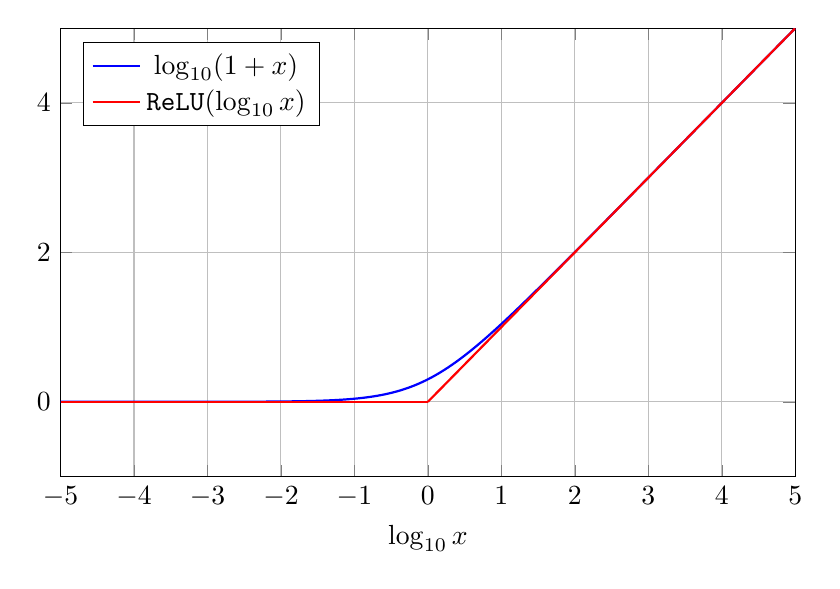
\begin{tikzpicture}
                \begin{axis}[
                    xlabel={$\log_{10} x$},
                    ylabel={},
                    legend pos=north west,
                    grid=both,
                    xmin=-5, xmax=5,
                    ymin=-1, ymax=5,
                    width=0.9\textwidth,
                    height=0.6\textwidth,
                ]
                % Plot log(1+10^x)
                \addplot[blue, thick, domain=-5:5, samples=200] {ln(1+10^x)/ln(10)};
                \addlegendentry{$\log_{10}(1+x)$}
                
                % Plot ReLU(log x) = max(0, log x)
                \addplot[red, thick, domain=-5:0, samples=50] {0};
                \addplot[red, thick, domain=0:5, samples=50] {x};
                \addlegendentry{$\mathtt{ReLU}(\log_{10} x)$}
                \end{axis}
            \end{tikzpicture}
        \end{figure}
        \end{columns}
    \end{frame}
    \begin{frame}{伯特图的绘制}
        伯特图的绘制几乎属于必考题型,也是比较简单和套路的一种考题。主要分为两个步骤:
        \uncover<2->{
            \begin{block}{第一步:求传函并因式分解}
                求出有理式形式的传递函数:$H_0\Rightarrow$幅频曲线最大值
                $$
                H(j\omega)=
                    H_0\frac{(1\pm j\frac{\omega}{\omega_{z1}})(1\pm j\frac{\omega}{\omega_{z2}})\cdots}{(1+j\frac{\omega}{\omega_{p1}})(1+j\frac{\omega}{\omega_{p2}})\cdots}
                $$
            \end{block}
        }
        \uncover<3->{
            \begin{block}{第二步: 零极点按照大小排序}
                \begin{itemize}
                    \item<4-> \textbf{幅频}\quad 碰到极点(斜率\texttt{+=})$-20\mathrm{dB/dec}$,碰到零点(斜率\texttt{+=}) $+20\mathrm{dB/dec}$。
                    \item <5-> \textbf{相频}\quad 极点滞后(相位在$0.1\sim10$倍频率内线性\textcolor{red}{\textbf{减少}})$90^\circ$,零点看左右,左\textcolor{red}{\textbf{超}}右\textcolor{red}{\textbf{滞}}$90^\circ$。
                    \item <5->$1+j\frac{\omega}{\omega_{z}}$左半平面,$1-j\frac{\omega}{\omega_{z}}$右半平面.即\textcolor{red}{$90^\circ$的正负号就是$j\dfrac{\omega}{\omega_z}$前面的正负号}。
                \end{itemize}
                \end{block}
        }
    \end{frame}
    \begin{frame}{伯特图的绘制}
        以上对于没有$0$零点的情况。如果有$0$零点怎么办?
        
        \pause

        有$0$零点时,传递函数形式为
        $$
        H(j\omega)=H_0\frac{(j\frac{\omega}{\omega_{z0}})^{m}(1\pm j\frac{\omega}{\omega_{z1}})(1\pm j\frac{\omega}{\omega_{z2}})\cdots}{(1+j\frac{\omega}{\omega_{p1}})(1+j\frac{\omega}{\omega_{p2}})\cdots}
        $$
        \pause
        
        由于频率取对数后,$0$零点对应到$-\infty$,因此幅频率曲线“天生”带一个$+m\times 20\mathrm{dB/dec}$的斜率,且相频曲线“天生”带相位$m\times 90^\circ$。

        \pause

        而回到之前的公式:
        \resizebox{1\textwidth}{!}{%
        $\displaystyle
        20\log\left|H(j\omega)\right|=20\log|H_0|+\sum_{i\in\text{零点}} 20\mathtt{Relu}\left(\log\frac{\omega}{\omega_{zi}}\right)-\sum_{i\in\text{极点}} 20\mathtt{Relu}\left(\log\frac{\omega}{\omega_{pi}}\right)\textcolor{red}{+20m\log\frac{\omega}{\omega_{z0}}}
        $}

        \pause

        可见,$0$零点对$\omega_{z0}$点的增益贡献恰好为$0\mathrm{dB}$。因此只需要巧妙地把$\omega_{z0}$放进通带即可。
    \end{frame}
    \begin{frame}{伯特图绘制}
        \begin{block}{例题}
            已知$H(j\omega)=-10^6\dfrac{j\omega\left(j\omega+5\times10^9\right)}{\left(j\omega+5\times10^6\right)\left(j\omega+1\times10^8\right)}$,绘制幅频特性和相频特性曲线。
            \end{block}
        \pause
        \begin{block}{解答}
            首先化简传递函数得到$H(j\omega)=(-10)\dfrac{j\omega\left(1+j\frac{\omega}{5\times10^9}\right)}{\left(1+j\frac{\omega}{5\times10^6}\right)\left(1+j\frac{\omega}{1\times10^8}\right)}$
            \pause

            然后列出零极点:
        \begin{itemize}
            \item 零点:$\omega_{z0}=0$, $\omega_{z1}=5\times10^9\mathrm{rad/s}$
            \item 极点:$\omega_{p1}=5\times10^6\mathrm{rad/s}$, $\omega_{p2}=1\times10^8\mathrm{rad/s}$
        \end{itemize}
        \end{block}
        
    \end{frame}
    \begin{frame}{伯特图绘制}
        $$H(j\omega)=(-10)\dfrac{j\omega\left(1+j\frac{\omega}{5\times10^9}\right)}{\left(1+j\frac{\omega}{5\times10^6}\right)\left(1+j\frac{\omega}{1\times10^8}\right)}$$
        \begin{block}{
            幅频特性曲线绘制
        }
        \pause
            \begin{table}
                \centering\resizebox{1\textwidth}{!}{%
                \begin{tabular}{c|c c c c}
                    \toprule
                    $\omega$ & $(0,5\times10^6]$ & $(5\times10^6, 1\times10^8]$ & $(1\times10^8, 5\times10^9]$ & $(5\times10^9, +\infty)$ \\
                    \midrule
                    斜率$(\mathrm{dB/dec})$ & $+20$ & $0$ & $-20$ & $0$ \\
                    \bottomrule
                \end{tabular}}
            \end{table}
        \pause
        求解平台增益:
\resizebox{1\textwidth}{!}{%
        $\displaystyle
        20\log\left|H(j\omega)\right|=20\log|H_0|+\sum_{i\in\text{零点}} 20\mathtt{Relu}\left(\log\frac{\omega}{\omega_{zi}}\right)-\sum_{i\in\text{极点}} 20\mathtt{Relu}\left(\log\frac{\omega}{\omega_{pi}}\right)\textcolor{red}{+20m\log\frac{\omega}{\omega_{z0}}}
        $}

        $(5\times10^6, 1\times10^8]$区间:($[5\times10^9,\infty)$区间不用再画)

        \resizebox{1\textwidth}{!}{%
        $\displaystyle
        H_{dB}=20\log 10+0-20\left(\log\omega-\log 5\times10^6\right)+20\left(\log\omega-\textcolor{red}{\log1}\right)=153.98\mathrm{dB}
        $}
        \end{block}

    \end{frame}
    \begin{frame}{伯特图绘制}
    \begin{block}{
        幅频特性曲线绘制
    }
    \begin{figure}
        \centering
        \resizebox{1\textwidth}{!}{
        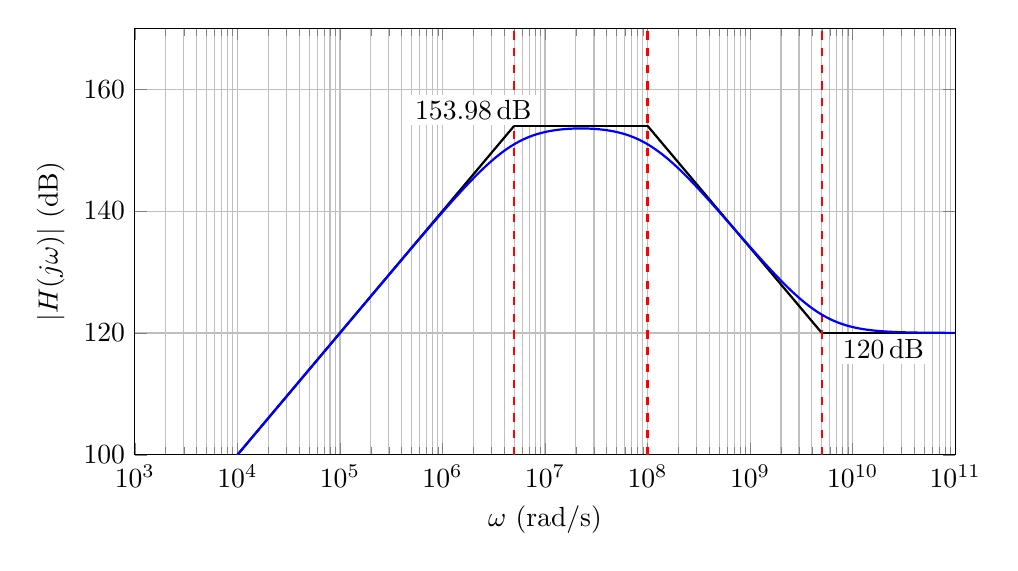
\begin{tikzpicture}
  \begin{semilogxaxis}[
    width=12cm,
    height=7cm,
    xlabel={$\omega\ \mathrm{(rad/s)}$},
    ylabel={$|H(j\omega)|\ \mathrm{(dB)}$},
    grid=both,
    xmin=1e3,
    xmax=1e11,
    ymin=100,
    ymax=170,
    log basis x=10,
  ]

    % ---------- 幅频渐近线 ----------

    % +20 dB/dec
    \addplot[
      thick,
      domain=1e3:5e6,
      samples=200
    ] {20*log10(x) + 20};

    % 平台 153.98 dB
    \addplot[
      thick,
      domain=5e6:1e8
    ] {153.98};

    % -20 dB/dec
    \addplot[
      thick,
      domain=1e8:5e9,
      samples=200
    ] {-20*log10(x) + 313.98};

    % 高频平台 120 dB
    \addplot[
      thick,
      domain=5e9:1e11
    ] {120};

    % ---------- 红色竖虚线:拐点 ----------

    \addplot[
      red,
      dashed,
      thick
    ] coordinates {(5e6,100) (5e6,170)};

    \addplot[
      red,
      dashed,
      thick
    ] coordinates {(1e8,100) (1e8,170)};

    \addplot[
      red,
      dashed,
      thick
    ] coordinates {(5e9,100) (5e9,170)};
    \addplot[
      blue,
      thick,
      domain=1e3:1e11,
      samples=600
    ]{20*log10(
  sqrt(100*(x*x*(1+(x/5e9)^2))/
  ((1+(x/5e6)^2)*(1+(x/1e8)^2)))
)};
    % ---------- 数值标注:平台高度 ----------

    \node[
      anchor=south,
      fill=white,
      inner sep=2pt
    ] at (axis cs:2e6,153.98)
    {$153.98\,\mathrm{dB}$};

    \node[
      anchor=north,
      fill=white,
      inner sep=2pt
    ] at (axis cs:2e10,120)
    {$120\,\mathrm{dB}$};

  \end{semilogxaxis}
\end{tikzpicture}}


    \end{figure}
    \end{block}
    \end{frame}
    \begin{frame}{伯特图绘制}
        $$H(j\omega)=(-10)\dfrac{j\omega\left(1+j\frac{\omega}{5\times10^9}\right)}{\left(1+j\frac{\omega}{5\times10^6}\right)\left(1+j\frac{\omega}{1\times10^8}\right)}$$
    \begin{block}{
        相频特性曲线绘制
    }
        \pause
        $0$频点:$-10$提供$180^\circ$相位,$j\omega$提供$90^\circ$相位,总计$270^\circ$相位。
        \pause
            \begin{table}
                \centering\resizebox{1\textwidth}{!}{%
                \begin{tabular}{c|c c c c}
                    \toprule
                    $\omega$ &$0$& $5\times10^5\to5\times10^7$ & $1\times10^7\to1\times10^9$ & $5\times10^8\to5\times10^{10}$  \\
                    \midrule
                    $\varphi(\mathrm{deg})$ & $270$ & $270\to180$ & $180\to90$&$90\to180$ \\
                    \bottomrule
                \end{tabular}}
            \end{table}
            \pause
            
            重叠的区间:取四边形对角线
        \end{block}
    \end{frame}
    \begin{frame}{伯特图绘制}
        \begin{block}{相频特性曲线绘制}
            \begin{figure}
  \centering
  \resizebox{1\linewidth}{!}{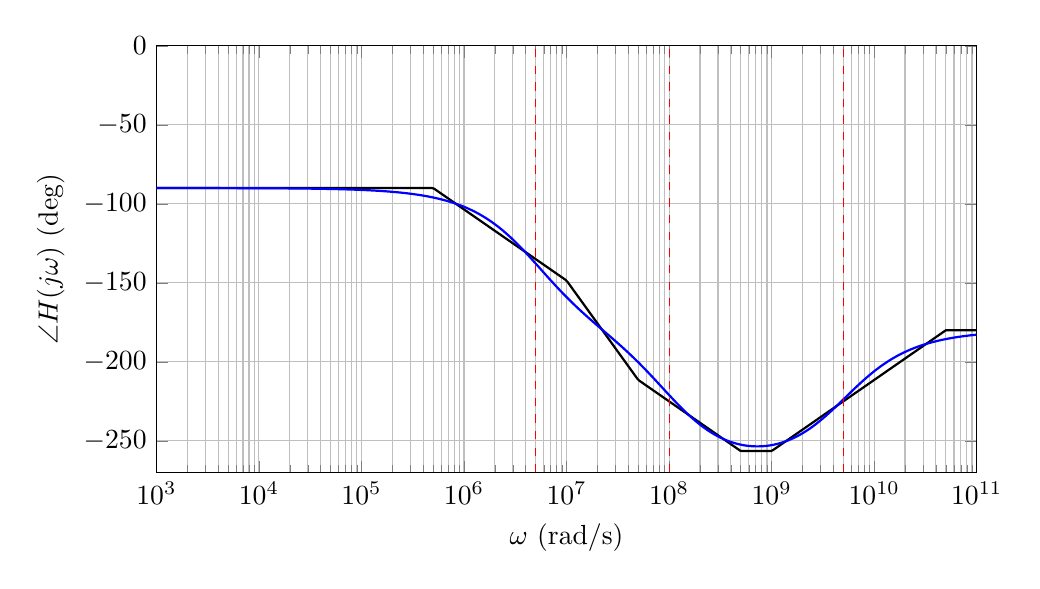
\begin{tikzpicture}
    \begin{semilogxaxis}[
      width=12cm,
      height=7cm,
      xlabel={$\omega\ \mathrm{(rad/s)}$},
      ylabel={$\angle H(j\omega)\ \mathrm{(deg)}$},
      grid=both,
      xmin=1e3,
      xmax=1e11,
      ymin=-270,
      ymax=0,
      log basis x=10,
      legend style={at={(0.02,0.02)},anchor=south west},
      declare function={
        % 一阶极点的伯特相位近似(单位:度)
        phiP(\w,\wzero) = 
          (\w <= 0.1*\wzero) ? 0 :
          ( (\w >= 10*\wzero) ? -90 :
            -45*(ln(\w/\wzero)/ln(10) + 1) );
        % 一阶零点的伯特相位近似(单位:度)
        phiZ(\w,\wzero) = 
          (\w <= 0.1*\wzero) ? 0 :
          ( (\w >= 10*\wzero) ?  90 :
             45*(ln(\w/\wzero)/ln(10) + 1) );
      },
    ]

      % ================== 伯特折线近似相位 ==================
      % 常数(-10)给 -180°,jω 给 +90°,其余用 phiP / phiZ 叠加
      \addplot[
        thick,
        domain=1e3:1e11,
        samples=400
      ]
      {
        -90
        + phiP(x,5e6)   % 极点 at 5e6
        + phiP(x,1e8)   % 极点 at 1e8
        + phiZ(x,5e9)   % 零点 at 5e9
      };
      

      % ================== 精确相位曲线 ==================
      % 注意:pgfmath 的 atan() 返回度数
      \addplot[
        blue,
        thick,
        domain=1e3:1e11,
        samples=600
      ]
      {
        -90
        + atan(x/5e9)
        - atan(x/5e6)
        - atan(x/1e8)
      };
      

      % ========== 可选:红色竖虚线标出拐点 ==========
      \foreach \w in {5e6,1e8,5e9}{
        \addplot[red,dashed]
          coordinates {(\w,-270) (\w,0)};
      }

    \end{semilogxaxis}
  \end{tikzpicture}}
\end{figure}

        \end{block}
    \end{frame}
\begin{frame}{滤波器分析}
    \remind{这些内容应当牢记!}
    $3\mathrm{dB}$: $H(s)=\frac{H_0}{\sqrt 2}$
\begin{block}{二阶滤波器的$3\mathrm{dB}$特性}
    \begin{columns}
        \column{.38\textwidth}
        \begin{center}
            二阶低通
        \end{center}
        \resizebox{1\textwidth}{!}{
        $\displaystyle
        \omega_{3\mathrm{dB}}=\begin{cases}
            \omega_0 & \xi=\frac{1}{\sqrt 2}\\
            \dfrac{1}{2\xi}&\xi\gg 1\\
            1.554\omega_0 & \xi\ll 1\\
        \end{cases}
        $}
        \column{.38\textwidth}
        \begin{center}
            二阶高通
        \end{center}
         \resizebox{1\textwidth}{!}{
        $\displaystyle
        \omega_{3\mathrm{dB}}=\begin{cases}
            \omega_0 & \xi=\frac{1}{\sqrt 2}\\
            2\xi&\xi\gg 1\\
            \dfrac{1}{1.554}\omega_0 & \xi\ll 1\\
        \end{cases}
        $}
        \column{.26\textwidth}
        \begin{center}
            二阶带阻/带通
        \end{center}
        \resizebox{1\textwidth}{!}{
            $\displaystyle\begin{aligned}
            BW_{3\mathrm{dB}}&=f_2-f_1=\dfrac{f_0}{Q}\\
            f_0&=\sqrt{f_1f_2}=\dfrac{\omega_0}{2\pi}\\
            Q&=\dfrac{1}{2\xi}
            \end{aligned}
            $}
    \end{columns}
\end{block}
\pause
\begin{block}{平坦特性}
    \begin{table}
        \centering
        \resizebox{0.55\textwidth}{!}{%
        \begin{tabular}{c|c c}
            \toprule
            $\xi$ & 名字 & 特性\\
            \midrule
            $0.707$ & 巴特沃斯 & 幅度最大平坦\\
            $0.866$ & 切比雪夫 & 群延时最大平坦\\
            $(0.707,1)$ & 最优二阶高/低通 & 快的阶跃响应\\
            \bottomrule
        \end{tabular}
        }
    \end{table}
\end{block}

\end{frame}
\begin{frame}{滤波器分析}
    \begin{block}{谐振现象}
        \remind{这些内容应当牢记!}
        \pause
        时域:体现为\textbf{振铃}现象,振铃时间$1.5QT$
        \pause

        频域:出现谐振峰($\Im(Z)=0/\Im(Y)=0$)
        \pause
        \begin{columns}
            \column{0.5\textwidth}
            \begin{center}
                低通系统
            \end{center}
            $$
            \begin{aligned}
                \omega_e&=\sqrt{1-2\xi^2}\omega_0\quad(\xi<0.707)\\
                A(\omega_e)&=\frac{1}{2\xi\sqrt{1-\xi^2}}H_0\\
                &\approx QH_0\quad(\xi\ll 0.707)
            \end{aligned}
            $$

            \column{0.5\textwidth}
            \begin{center}
                高通系统
            \end{center}
            $$
            \begin{aligned}
                \omega_e&=\frac{1}{\sqrt{1-2\xi^2}}\omega_0\quad(\xi<0.707)\\
                A(\omega_e)&=\frac{1}{2\xi\sqrt{1-\xi^2}}H_0\\
                &\approx QH_0\quad(\xi\ll 0.707)
            \end{aligned}
            $$
        \end{columns}
        \pause

        对于高$Q$系统,有$\omega_e\approx \omega_0, A(\omega_e)\approx QH_0$。
            

        
    \end{block}
\end{frame}
\begin{frame}{滤波器分析}
\begin{block}{例题(2024年T10回忆版)}
    \begin{columns}
        \column{0.55\textwidth}
        右侧电路中,NMOS在该偏置下$g_m=40\mathrm{mS}$,$r_{ds}=\infty$,全耦合变压器的匝数比为$1:2$, 初级绕组电感$L=40\mu \mathrm{H}$,电容$C=100\mathrm{pF}$,负载电阻$R=2k\mathrm{\Omega}$。假设输入信号$v_i$为交流小信号。则系统的传递函数$H_v(s)=\frac{v_o}{v_i}$ 为[\qquad]。这是一个[\qquad]滤波器(低通/高通/带通/带阻),其3dB频点(高低通)或带宽(带通/带阻)为[\qquad]。
        \column{0.4\textwidth}
        \begin{figure}[!ht]
\centering
\resizebox{1\textwidth}{!}{%
\begin{circuitikz}
\tikzstyle{every node}=[font=\LARGE]
\draw (10,14.5) to[C,l={ \LARGE $C$}] (10,17);
\draw (11.25,17) to[L ] (11.25,14.5);
\draw (12.5,14.5) to[L ] (12.5,17);
\draw (13.75,17) to[R,l={ \LARGE $R$}] (13.75,14.5);
\draw (10,17) to[short] (11.25,17);
\draw (10,14.5) to[short] (11.25,14.5);
\draw (10.5,12.5) to[Tnmos, transistors/scale=1.02] (10.5,14.5);
\draw (10.5,12.5) to (10.5,12.25) node[sground]{};
\draw (12.5,17) to[short] (13.75,17);
\draw (12.5,14.5) to[short] (13.75,14.5);
\draw (13.75,17) to[short, -o] (14.75,17) ;
\draw (8.75,13.5) to[sinusoidal voltage source, sources/symbol/rotate=auto] (8.75,12);
\draw (8.75,13.5) to[short] (9.5,13.5);
\draw (8.75,10.75) to (8.75,10.5) node[sground]{};
\draw (13,14.5) to (13,14.25) node[sground]{};
\draw [short] (10.25,18.25) -- (10.75,18.25);
\draw (10.5,18.25) to[short] (10.5,17);
\node [font=\LARGE] at (10.5,18.75) {$V_{DD}$};
\node [font=\LARGE] at (11.75,17.25) {$1:2$};
\node [font=\LARGE] at (12,14.75) {$k=1$};
\node at (11.5,16.75) [circ] {};
\node at (12.25,16.75) [circ] {};
\node [font=\LARGE] at (10.75,15.25) {$L$};
\node [font=\LARGE] at (15.25,17.25) {$v_o$};
\node [font=\LARGE] at (8,13) {$v_i$};
\draw (8.75,12) to[battery ,l={ \LARGE $V_G$}] (8.75,10.75);
\end{circuitikz}
}%
\end{figure}
    \end{columns}
\end{block}
\end{frame}
\begin{frame}{滤波器分析}
    \begin{block}{解答}
        画出其小信号模型:
\pause

\begin{figure}[!ht]
\centering
\resizebox{.5\textwidth}{!}{%
\begin{circuitikz}
\tikzstyle{every node}=[font=\LARGE]
\draw (10,14.5) to[C,l={ \LARGE $C$}] (10,17);
\draw (11.25,17) to[L ] (11.25,14.5);
\draw (12.5,14.5) to[L ] (12.5,17);
\draw (13.75,17) to[R,l={ \LARGE $R$}] (13.75,14.5);
\draw (10,17) to[short] (11.25,17);
\draw (10,14.5) to[short] (11.25,14.5);
\draw (12.5,17) to[short] (13.75,17);
\draw (12.5,14.5) to[short] (13.75,14.5);
\draw (13.75,17) to[short, -o] (14.75,17) ;
\node [font=\LARGE] at (11.75,17.25) {$1:2$};
\node [font=\LARGE] at (11.75,18) {$k=1$};
\node at (11.5,14.75) [circ] {};
\node at (12.25,16.75) [circ] {};
\node [font=\LARGE] at (10.75,15.25) {$L$};
\node [font=\LARGE] at (15.25,17.25) {$v_o$};

\draw (8.25,17) to[short] (10,17);
\draw (8.25,14.5) to[short] (12.5,14.5);
\draw (6.75,17) to[short, -o] (5.75,17) ;
\draw (8.25,14.5) to[short] (6.5,14.5);
\draw (6.5,14.5) to[short, -o] (5.75,14.5) ;
\node [font=\LARGE] at (5.75,15.75) {$v_i$};
\draw (8.25,17) to[american current source] (8.25,14.5);
\node [font=\LARGE] at (7.25,15.75) {$g_mv_i$};
\end{circuitikz}
}%

\end{figure}

\pause

等效掉互感:注意变压比$M:L_2=kN_1N_2:N_2^2=kN_1:N_2=1:2$
\begin{figure}[!ht]
\centering
\resizebox{0.6\textwidth}{!}{%
\begin{circuitikz}
\tikzstyle{every node}=[font=\LARGE]
\draw (10,14.5) to[C,l={ \LARGE $C$}] (10,17);
\draw (13,17) to[L ] (13,14.5);
\draw (14.25,14.5) to[L ] (14.25,17);
\draw (15.5,17) to[R,l={ \LARGE $R$}] (15.5,14.5);
\draw (11.75,17) to[short] (13,17);
\draw (11.75,14.5) to[short] (13,14.5);
\draw (14.25,17) to[short] (15.5,17);
\draw (14.25,14.5) to[short] (15.5,14.5);
\draw (15.5,17) to[short, -o] (16.5,17) ;
\node [font=\LARGE] at (13.5,17.5) {$M:L_2$};
\node at (13.25,14.75) [circ] {};
\node at (14,16.75) [circ] {};
\node [font=\LARGE] at (17,17.25) {$v_o$};

\draw (8.25,17) to[short] (10,17);
\draw (10,14.5) to[short] (14.25,14.5);
\draw (6.75,17) to[short, -o] (5.75,17) ;
\draw (8.25,14.5) to[short] (6.5,14.5);
\draw (6.5,14.5) to[short, -o] (5.75,14.5) ;
\node [font=\LARGE] at (5.75,15.75) {$v_i$};
\draw (8.25,17) to[american current source] (8.25,14.5);
\node [font=\LARGE] at (7.25,15.75) {$g_mv_i$};
\draw (8.25,14.5) to[short] (10,14.5);
\draw (11.75,17) to[L,l={ \LARGE $L$} ] (11.75,14.5);
\draw (10,17) to[short] (11.75,17);
\draw (9,14.5) to (9,14.25) node[sground]{};
\end{circuitikz}
}
\end{figure}
    \end{block}
\end{frame}
\begin{frame}{滤波器分析}
    \begin{block}{解答}
        反射电阻:
        $R'=\left(\dfrac{N_1}{N_2}\right)^2R=\dfrac{1}{4}R=500\Omega$
        \begin{figure}[!t]
\centering
\resizebox{0.6\textwidth}{!}{%
\begin{circuitikz}
\tikzstyle{every node}=[font=\LARGE]
\draw (9.75,14.5) to[C,l={ \LARGE $C$}] (9.75,17);
\draw (13,17) to[L ] (13,14.5);
\draw (14.25,14.5) to[L ] (14.25,17);
\draw (10.5,17) to[R,l={ \LARGE $R'$}] (10.5,14.5);
\draw (11.75,17) to[short] (13,17);
\draw (11.75,14.5) to[short] (13,14.5);
\draw (14.25,17) to[short] (15.5,17);
\draw (15.5,17) to[short, -o] (16.5,17) ;
\node [font=\LARGE] at (13.5,17.5) {$M:L_2$};
\node at (13.25,14.75) [circ] {};
\node at (14,16.75) [circ] {};
\node [font=\LARGE] at (17,17.25) {$v_o$};

\draw (8.25,17) to[short] (10,17);
\draw (10,14.5) to[short] (14.25,14.5);
\draw (6.75,17) to[short, -o] (5.75,17) ;
\draw (8.25,14.5) to[short] (6.5,14.5);
\draw (6.5,14.5) to[short, -o] (5.75,14.5) ;
\node [font=\LARGE] at (5.75,15.75) {$v_i$};
\draw (8.25,17) to[american current source] (8.25,14.5);
\node [font=\LARGE] at (7.25,15.75) {$g_mv_i$};
\draw (8.25,14.5) to[short] (10,14.5);
\draw (11.75,17) to[L,l={ \LARGE $L$} ] (11.75,14.5);
\draw (10,17) to[short] (11.75,17);
\draw (9,14.5) to (9,14.25) node[sground]{};


\end{circuitikz}
}%

\end{figure}

\pause
则传递函数为:
\resizebox{\textwidth}{!}{
$\displaystyle
\begin{aligned}
H_v(s)&=-g_m\cdot\left(\frac{1}{sC}\parallel R'\parallel sL\right)\cdot(-2)\\
&=\frac{2g_mR'}{sC+1/R'+1/sL}=\frac{(2g_mR'/C)s}{s^2+(1/CR')s+(1/LC)}=\frac{4\times10^{11}s}{s^2+2\times10^7s+2.5\times10^{14}}\\
\end{aligned}
$}

    \end{block}
\end{frame}
\begin{frame}
    \begin{block}{解答}
$$
H_v(s)=\frac{4\times10^{11}s}{s^2+2\times10^7s+2.5\times10^{14}}=H_0\frac{2\xi\omega_0s}{s^2+2\xi\omega_0s+\omega_0^2}
$$
\pause
$$
\therefore\begin{cases}
\omega_0=1.58\times10^7\mathrm{rad/s}\\
\xi=0.632\\
H_0=2\times10^4
\end{cases}
$$
\pause
$$
\therefore\text{带通滤波器,}BW=\dfrac{\omega_0}{2\pi Q}=\dfrac{2\xi\omega_0}{2\pi}=3.18\mathrm{MHz}
$$
    \end{block}
    \pause
    \begin{block}{提示}
        请务必重温一下上个学期的内容!同时CAD作业也可能作为考试题目!
    \end{block}
\end{frame}
\begin{frame}{频点估算}
    频点估算即根据各个电容的频点估算总体的高低端$3\mathrm{dB}$频点。需要记住口诀

    \begin{center}
        \textcolor{TsinghuaPurple}{\emph{
        高通开路算频点,低通短路看时间}
        }
    \end{center}
    \pause

    低端$3\mathrm{dB}$频点由高通电容(耦合电容、旁路电容)决定,使用开路法计算。即
    $$
    f_{L,3\mathrm{dB}}\approx f_{L1}+f_{L2}+\cdots=\frac{1}{2\pi}\left(\frac{1}{R_1C_1}+\frac{1}{R_2C_2}+\cdots\right)
    $$
    其中$R_i$为除了$C_i$外电容全部开路后,$C_i$看到的等效电阻。

    \pause
    高端$3\mathrm{dB}$频点由低通电容(通常是晶体管寄生电容)决定,使用短路法计算。即
    $$
    f_{L,3\mathrm{dB}}\approx\frac{1}{2\pi(\tau_{H1}+\tau_{H2}+\cdots)}=\frac{1}{2\pi}\frac{1}{R_1C_1+R_2C_2+\cdots}
    $$
    其中$R_i$为除了$C_i$外电容全部短路后,$C_i$看到的等效电阻。

\end{frame}
\subsection{神秘小技巧}
\begin{frame}{阻抗匹配}
    借助双向无损网络阻抗匹配。最大功率匹配(共轭匹配)条件:$Z_L=Z_S^\ast$, 需要记住口诀(他可能直接考这句话默写)
    \begin{center}
        \textcolor{TsinghuaPurple}{并大串小Q相等
        }
    \end{center}
    \pause

    也就是$R$大的一侧并东西,$R$小的一侧串东西。其中品质因数
    $$
    Q=\underbrace{\dfrac{\text{串联电抗}}{\text{串联电阻}}=\dfrac{\text{并联电纳}}{\text{并联电导}}}_{\text{局部}}=\underbrace{\sqrt{\frac{R_P}{R_S}-1}}_{\text{整体}}
    $$
\end{frame}
\begin{frame}{串并等效}
    当$Q\gg 1$时在\textcolor{red}{谐振频点附近},可以做如下等效:
\begin{figure}[!ht]
\centering
\resizebox{.7\textwidth}{!}{%
\begin{circuitikz}
\tikzstyle{every node}=[font=\LARGE]
\draw (7.5,16) to[R,l={ \LARGE $R$}] (10,16);
\draw (10,16) to[L,l={ \LARGE $L$} ] (10,13.5);
\draw (7.5,16) to[short, -o] (6.25,16) ;
\draw (10,13.5) to[short, -o] (6.25,13.5) ;
\draw (17.5,16) to[L,l={ \LARGE $L$} ] (17.5,13.5);
\draw (16.25,13.5) to[R,l={ \LARGE $Q^2R$}] (16.25,16);
\draw (17.5,16) to[short, -o] (13.75,16) ;
\draw (17.5,13.5) to[short, -o] (13.75,13.5) ;
\draw [<->, >=Stealth] (11.75,14.75) -- (12.75,14.75);
\draw (7.5,12.25) to[R,l={ \LARGE $R$}] (10,12.25);
\draw (7.5,12.25) to[short, -o] (6.25,12.25) ;
\draw (10,9.75) to[short, -o] (6.25,9.75) ;
\draw (16.25,9.75) to[R,l={ \LARGE $Q^2R$}] (16.25,12.25);
\draw (17.5,12.25) to[short, -o] (13.75,12.25) ;
\draw (17.5,9.75) to[short, -o] (13.75,9.75) ;
\draw [<->, >=Stealth] (11.75,11) -- (12.75,11);
\draw (10,12.25) to[C,l={ \LARGE $C$}] (10,9.75);
\draw (17.5,12.25) to[C,l={ \LARGE $C$}] (17.5,9.75);
\end{circuitikz}
}%
\end{figure}
\end{frame}
\begin{frame}{部分接入法}
    当$Q\gg 1$时在\textcolor{red}{谐振频点附近},可以做如下等效:($p$:分压比(接入系数))
    \begin{figure}[!ht]
\centering
\resizebox{.8\textwidth}{!}{%
\begin{circuitikz}
\tikzstyle{every node}=[font=\LARGE]
\draw (7.5,16) to[short, -o] (6.25,16) ;
\draw (7.5,16) to[C,l={ \LARGE $C_1$}] (7.5,14.25);
\draw (7.5,12.25) to[C,l={ \LARGE $C_2$}] (7.5,14.25);
\draw (7.5,12.25) to[short, -o] (6.25,12.25) ;
\draw (8.75,14) to[R,l={ \LARGE $R$}] (8.75,12.25);
\draw (7.5,12.25) to[short] (8.75,12.25);
\draw (8.75,14) to[short] (7.5,14);
\draw (13.25,16) to[short, -o] (10.75,16) ;
\draw (13.25,16) to[C] (13.25,14.25);
\draw (13.25,14.25) to[C] (13.25,12.25);
\draw (11.25,12.25) to[short, -o] (10.75,12.25) ;
\draw (13.25,12.25) to[R] (11.25,12.25);
\draw (16.75,16) to[short, -o] (15.5,16) ;
\draw (16.75,16) to[C,l={ \LARGE $C_1$}] (16.75,14.25);
\draw (16.75,14.25) to[C,l={ \LARGE $C_2$}] (16.75,12.25);
\draw (16.75,12.25) to[short, -o] (15.5,12.25) ;
\draw (18,16) to[R,l={ \LARGE $\frac{R}{p^2}$}] (18,12.25);
\draw (16.75,12.25) to[short] (18,12.25);
\draw (18,16) to[short] (16.75,16);
\draw [<->, >=Stealth] (9.5,14) -- (10.5,14);
\node [font=\LARGE] at (11,13.5) {};
\draw [<->, >=Stealth] (14.25,14) -- (15.25,14);
\node [font=\LARGE] at (4,14) {$p=\frac{C_1}{C_1+C_2}$};
\draw (7.5,11.5) to[short, -o] (6.25,11.5) ;
\draw (7.5,7.75) to[short, -o] (6.25,7.75) ;
\draw (8.75,9.5) to[R,l={ \LARGE $R$}] (8.75,7.75);
\draw (7.5,7.75) to[short] (8.75,7.75);
\draw (8.75,9.5) to[short] (7.5,9.5);
\draw (13.25,11.5) to[short, -o] (10.75,11.5) ;
\draw (11.25,7.75) to[short, -o] (10.75,7.75) ;
\draw (13.25,7.75) to[R] (11.25,7.75);
\draw (16.75,11.5) to[short, -o] (15.5,11.5) ;
\draw (16.75,7.75) to[short, -o] (15.5,7.75) ;
\draw (18,11.5) to[R,l={ \LARGE $\frac{R}{p^2}$}] (18,7.75);
\draw (16.75,7.75) to[short] (18,7.75);
\draw (18,11.5) to[short] (16.75,11.5);
\draw [<->, >=Stealth] (9.5,9.5) -- (10.5,9.5);
\node [font=\LARGE] at (11,9) {};
\draw [<->, >=Stealth] (14.25,9.5) -- (15.25,9.5);
\node [font=\LARGE] at (4,9.5) {$p=\frac{L_2}{L_1+L_2}$};
\draw (7.5,11.5) to[L,l={ \LARGE $L_1$} ] (7.5,9.5);
\draw (7.5,9.5) to[L,l={ \LARGE $L_2$} ] (7.5,7.75);
\draw (13.25,11.5) to[L,l={ \LARGE $L_1$} ] (13.25,9.75);
\draw (13.25,9.75) to[L,l={ \LARGE $L_2$} ] (13.25,7.75);
\draw (16.75,11.5) to[L,l={ \LARGE $L_1$} ] (16.75,9.75);
\draw (16.75,9.75) to[L,l={ \LARGE $L_2$} ] (16.75,7.75);
\end{circuitikz}
}%


\end{figure}
\end{frame}
\subsection{反馈}
\begin{frame}{负反馈}
负反馈放大器的分析流程:\begin{enumerate}
    \item 分析连接方式,反馈网络直连放大网络输出则为并联,否则为串联;
    \item 分析开环放大器参量。反馈网络画两遍,输入端反馈源置零,输出端反馈负载置零。求$r_{in},r_{out}$需要输入/输出端置0,求$A$需要负载置0。
    \item 求反馈系数:加x求y
    \item 代入公式$A=\frac{A_o}{1+T}$,$w_{in,c}=(1+T)w_{in,o}$,$w_{out,c}=(1+T)w_{out,o}$
\end{enumerate}
\pause
\begin{figure}
    \centering
    \includegraphics[width=0.6\textwidth]{figures/feedback.png}
\end{figure}
\remind{反馈网络的21元素被忽略了,因为增益相对前馈很小}
\end{frame}
\begin{frame}{负反馈}
    \begin{block}{例题}
        已知运算放大器电压增益$A_{v0}$,BJT的跨导为$g_m$, 求电路的输入输出电阻和增益($r_{bc}\,,r_{ce}\to\infty$)。
        \begin{figure}[!ht]
\centering
\resizebox{.4\textwidth}{!}{%
\begin{circuitikz}
\tikzstyle{every node}=[font=\LARGE]
\draw (12.25,17.25) node[op amp,scale=1] (opamp2) {};
\draw (opamp2.+) to[short] (10.75,16.75);
\draw  (opamp2.-) to[short] (10.75,17.75);
\draw (13.45,17.25) to[short](13.75,17.25);
\draw (14.75,16) to[Tnpn, transistors/scale=1.19] (14.75,18.5);
\draw (14.75,18.5) to[R=$R_C$] (14.75,20.25);
\draw (10.75,16.75) to[short] (10,16.75);
\draw (10,16.75) to[short] (10,18.5);
\draw (10,18.5) to[short] (14.75,18.5);
\draw (10.75,17.75) to[short, -o] (8.75,17.75) ;
\draw (14.75,20.25) to[short] (14.75,20.75);
\draw [short] (14.5,20.75) -- (15,20.75);
\node [font=\LARGE] at (14.5,21.25) {$V_{CC}$};
\draw (10,14.75) to[short, -o] (8.75,14.75) ;
\draw (14.75,16) to[short, -o] (15.75,16) ;
\draw (14.75,14.75) to[short, -o] (15.75,14.75) ;
\draw (14.75,14.75) to[short] (14.75,13.75);
\draw [short] (14.5,13.75) -- (15,13.75);
\node [font=\LARGE] at (14.5,13.25) {$V_{EE}$};
\draw (10,14.75) to (10,14.25) node[sground]{};
\node [font=\LARGE] at (8.5,16.25) {in};
\node [font=\LARGE] at (16.25,15.5) {out};
\node [font=\LARGE] at (15,17.25) {$T$};
\end{circuitikz}
}%

\end{figure}
    \end{block}
    \pause
    提示:$T$是CC组态$\Rightarrow$电压缓冲器,电流放大器!
\end{frame}

\begin{frame}{负反馈}
    \begin{block}{解答}
首先把小信号模型代入进去,然后把运放和晶体管“翻”过来。

\pause
\begin{figure}[!ht]
\centering
\resizebox{1\textwidth}{!}{%
\begin{circuitikz}
\tikzstyle{every node}=[font=\LARGE]
\draw (12.25,17.25) node[op amp,scale=1] (opamp2) {};
\draw (opamp2.+) to[short] (10.75,16.75);
\draw  (opamp2.-) to[short] (10.75,17.75);
\draw (13.45,17.25) to[short](13.75,17.25);
\draw (14.75,16) to[Tnpn, transistors/scale=1.19] (14.75,18.5);
\draw (14.75,20.25) to[R,l={ \LARGE $R_C$}] (14.75,18.5);
\draw (10.75,16.75) to[short] (10,16.75);
\draw (10,16.75) to[short] (10,18.5);
\draw (10,18.5) to[short] (14.75,18.5);
\draw (10.75,17.75) to[short, -o] (8.75,17.75) ;
\draw (10,14.75) to[short, -o] (8.75,14.75) ;
\draw (14.75,16) to[short, -o] (15.75,16) ;
\draw (14.75,14.75) to[short, -o] (15.75,14.75) ;
\draw (10,14.75) to (10,14.25) node[sground]{};
\node [font=\LARGE] at (8.5,16.25) {in};
\node [font=\LARGE] at (16.25,15.5) {out};
\node [font=\LARGE] at (15,17.25) {$T$};
\draw (14,20) to (14,19.75) node[sground]{};
\draw (12.25,17.25) node[op amp,scale=1] (opamp2) {};
\draw (opamp2.+) to[short] (10.75,16.75);
\draw  (opamp2.-) to[short] (10.75,17.75);
\draw (13.45,17.25) to[short](13.75,17.25);
\draw (12.25,17.25) node[op amp,scale=1] (opamp2) {};
\draw (opamp2.+) to[short] (10.75,16.75);
\draw  (opamp2.-) to[short] (10.75,17.75);
\draw (13.45,17.25) to[short](13.75,17.25);
\draw (14.75,14.75) to (14.75,14.25) node[sground]{};
\draw (14,20) to[short] (14,20.5);
\draw (14,20.5) to[short] (14.75,20.5);
\draw (14.75,20.5) to[short] (14.75,20);
\draw (24,20.25) to[R,l={ \LARGE $R_C$}] (24,18.5);
\draw (19.25,16.75) to[short] (19.25,18.5);
\draw (19.25,18.5) to[short] (24,18.5);
\draw (19.25,17.75) to[short, -o] (18,17.75) ;
\draw (19.25,14.75) to[short, -o] (18,14.75) ;
\draw (24,16) to[short, -o] (25,16) ;
\draw (24,14.75) to[short, -o] (25,14.75) ;
\draw (19.25,14.75) to (19.25,14.25) node[sground]{};
\node [font=\LARGE] at (17.75,16.25) {in};
\node [font=\LARGE] at (25.5,15.5) {out};
\draw (23.25,20) to (23.25,19.75) node[sground]{};
\draw (12.25,17.25) node[op amp,scale=1] (opamp2) {};
\draw (opamp2.+) to[short] (10.75,16.75);
\draw  (opamp2.-) to[short] (10.75,17.75);
\draw (13.45,17.25) to[short](13.75,17.25);
\draw (12.25,17.25) node[op amp,scale=1] (opamp2) {};
\draw (opamp2.+) to[short] (10.75,16.75);
\draw  (opamp2.-) to[short] (10.75,17.75);
\draw (13.45,17.25) to[short](13.75,17.25);
\draw (24,14.75) to (24,14.25) node[sground]{};
\draw (23.25,20) to[short] (23.25,20.5);
\draw (23.25,20.5) to[short] (24,20.5);
\draw (24,20.5) to[short] (24,20);
\draw (21.75,18) to[american voltage source] (21.75,16.25);
\draw [->, >=Stealth] (20,17) -- (20,17.5);
\node [font=\LARGE] at (20.5,17.25) {$v_d$};
\node [font=\LARGE] at (21,16.5) {$A_vv_d$};
\draw (21.75,16.25) to (21.75,16) node[sground]{};
\draw (24,18.5) to[american current source,l={ \LARGE $g_m v_{be}$}] (24,16);
\draw (19.25,17.75) to[short, -o] (20,17.75) ;
\draw (19.25,16.75) to[short, -o] (20,16.75) ;
\draw (24,16) to[short, -o] (23,16) ;
\draw (21.75,18) to[short, -o] (23,18) ;
\draw [->, >=Stealth] (23,17.75) -- (23,16.25);
\node [font=\LARGE] at (22.5,16.75) {$v_{be}$};
\draw (30.5,16.5) to[R,l={ \LARGE $R_C$}] (30.5,14.75);
\draw (28.25,19) to[short, -o] (27,19) ;
\draw (33,19) to[short, -o] (34,19) ;
\node [font=\LARGE] at (27,16.75) {in};
\node [font=\LARGE] at (34.5,16.75) {out};
\draw (12.25,17.25) node[op amp,scale=1] (opamp2) {};
\draw (opamp2.+) to[short] (10.75,16.75);
\draw  (opamp2.-) to[short] (10.75,17.75);
\draw (13.45,17.25) to[short](13.75,17.25);
\draw (12.25,17.25) node[op amp,scale=1] (opamp2) {};
\draw (opamp2.+) to[short] (10.75,16.75);
\draw  (opamp2.-) to[short] (10.75,17.75);
\draw (13.45,17.25) to[short](13.75,17.25);
\draw (30.5,19) to[american voltage source] (30.5,17.5);
\draw [->, >=Stealth] (29,18.75) -- (29,18.25);
\node [font=\LARGE] at (29.5,18.5) {$v_d$};
\node [font=\LARGE] at (31.75,18.25) {$-A_vv_d$};
\draw (30.5,17.5) to (30.5,17.25) node[sground]{};
\draw (28.25,19) to[short, -o] (29,19) ;
\draw (28.25,18) to[short, -o] (29,18) ;
\draw (30.5,14.75) to[short, -o] (27,14.75) ;
\draw (30.5,14.75) to[short, -o] (34,14.75) ;
\draw [->, >=Stealth] (31.25,19) -- (32.25,19);
\node [font=\LARGE] at (31.75,19.75) {$v_{be}$};
\draw (28.25,18) to[short] (28.25,16.5);
\draw (28.25,16.5) to[short] (30.5,16.5);
\draw (29.25,14.75) to (29.25,14.25) node[sground]{};
\draw (12.25,17.25) node[op amp,scale=1] (opamp2) {};
\draw (opamp2.+) to[short] (10.75,16.75);
\draw  (opamp2.-) to[short] (10.75,17.75);
\draw (13.45,17.25) to[short](13.75,17.25);
\draw (12.25,17.25) node[op amp,scale=1] (opamp2) {};
\draw (opamp2.+) to[short] (10.75,16.75);
\draw  (opamp2.-) to[short] (10.75,17.75);
\draw (13.45,17.25) to[short](13.75,17.25);
\draw (12.25,17.25) node[op amp,scale=1] (opamp2) {};
\draw (opamp2.+) to[short] (10.75,16.75);
\draw  (opamp2.-) to[short] (10.75,17.75);
\draw (13.45,17.25) to[short](13.75,17.25);
\draw (30.5,16.5) to[short] (33,16.5);
\draw (30.5,19) to[short, -o] (31,19) ;
\draw (33,19) to[short, -o] (32.5,19) ;
\draw (33,16.5) to[american current source] (33,19);
\node [font=\LARGE] at (34.25,17.75) {$g_mv_{be}$};
\end{circuitikz}
}%
\end{figure}
\pause

显然这是个\textcolor{red}{串串负反馈}.
    \end{block}

\end{frame}

\begin{frame}{负反馈}
    \begin{block}{解答}
        求解开环放大器的输入输出电阻
    \begin{columns}
        \column{0.46\textwidth}
        \begin{figure}[!t]
\centering
\resizebox{.9\textwidth}{!}{%
\begin{circuitikz}
\tikzstyle{every node}=[font=\LARGE]
\draw (29.25,16.5) to[R,l={ \LARGE $R_C$}] (29.25,14.75);
\draw (28.25,19) to[short, -o] (27,19) ;
\draw (33,19) to[short, -o] (34,19) ;
\node [font=\LARGE] at (27,16.75) {in};
\node [font=\LARGE] at (34.5,16.75) {out};

\draw (30.5,19) to[american voltage source] (30.5,17.5);
\draw [->, >=Stealth] (29,18.75) -- (29,18.25);
\node [font=\LARGE] at (29.5,18.5) {$0$};
\node [font=\LARGE] at (31.25,18.25) {$0$};
\draw (30.5,17.5) to (30.5,17.25) node[sground]{};
\draw (28.25,19) to[short, -o] (29,19) ;
\draw (28.25,18) to[short, -o] (29,18) ;
\draw (29.25,14.75) to[short, -o] (27,14.75)--(27,19) ;
\draw (32,14.75) to[short, -o] (34,14.75) ;
\draw [->, >=Stealth] (31.25,19) -- (32.25,19);
\node [font=\LARGE] at (31.75,19.5) {$v_{be}=-v_{out}$};
\draw (28.25,18) to[short] (28.25,16.5);
\draw (28.25,16.5) to[short] (29.25,16.5);
\draw (28.5,14.75) to (28.5,14.25) node[sground]{};
\draw (30.5,19) to[short, -o] (31,19) ;
\draw (33,19) to[short, -o] (32.5,19) ;
\draw (33,19) to[american current source] (33,16.5);
\node [font=\LARGE] at (34.25,17.75) {$g_mv_{out}$};
\draw (32,16.5) to[R,l={ \LARGE $R_C$}] (32,14.75);
\draw (33,14.75) to (33,14.25) node[sground]{};
\draw (32,16.5) to[short] (33,16.5);
\end{circuitikz}
}%

\end{figure}
\pause
$$
\begin{aligned}
    i_{out}&=g_mv_{out}\\
    \pause
r_{out,o}&=\frac{v_{out}}{i_{out}}=\frac{1}{g_m}\\
\end{aligned}
$$
\pause
\column{0.46\textwidth}
\begin{figure}[!t]
\centering
\resizebox{1\textwidth}{!}{%
\begin{circuitikz}
\tikzstyle{every node}=[font=\LARGE]
\draw (29.25,16.5) to[R,l={ \LARGE $R_C$}] (29.25,14.75);
\draw (28.25,19) to[short, -o] (27,19) ;
\draw (33,19) to[short, -o] (34,19) ;
\node [font=\LARGE] at (27.5,16.75) {in};
\node [font=\LARGE] at (34.5,16.75) {out};

\draw (30.5,19) to[american voltage source] (30.5,17.5);
\draw [->, >=Stealth] (29,18.75) -- (29,18.25);
\node [font=\LARGE] at (29.5,18.5) {$v_d$};
\node [font=\LARGE] at (31.75,18.25) {$-A_vv_d$};
\draw (30.5,17.5) to (30.5,17.25) node[sground]{};
\draw (28.25,19) to[short, -o] (29,19) ;
\draw (28.25,18) to[short, -o] (29,18) ;
\draw (29.25,14.75) to[short, -o] (27,14.75) ;
\draw (32,14.75) to[short, -o] (34,14.75) ;
\draw [->, >=Stealth] (31.25,19) -- (32.25,19);
\node [font=\LARGE] at (31.75,19.75) {$v_{be}$};
\draw (28.25,18) to[short] (28.25,16.5);
\draw (28.25,16.5) to[short] (29.25,16.5);
\draw (28.5,14.75) to (28.5,14.25) node[sground]{};

\draw (30.5,19) to[short, -o] (31,19) ;
\draw (33,19) to[short, -o] (32.5,19) ;
\draw (33,16.5) to[american current source] (33,19);
\node [font=\LARGE] at (32.25,17.25) {$g_mv_{be}$};
\draw (32,16.5) to[R,l={ \LARGE $R_C$}] (32,14.75);
\draw (33,14.75) to (33,14.25) node[sground]{};
\draw (32,16.5) to[short] (33,16.5);
\draw (34,19) to[short] (34,14.75);
\draw [->, >=Stealth] (34,18) -- (34,17.5);
\node [font=\LARGE] at (34.5,17.5) {$i_{out}$};
\draw [->, >=Stealth] (27,18.5) -- (27,15.25);
\node [font=\LARGE] at (26.25,16.75) {$v_{in}$};
\end{circuitikz}
}%

\end{figure}
\pause
$$
r_{in,o}=\infty
$$
    \end{columns}

\end{block}
\end{frame}
\begin{frame}{负反馈}
    \begin{block}{解答}
        求解开环放大器的增益(压控流源放大器应该求$G_{m0}$)

        \begin{columns}
        \column{0.4\textwidth}
\begin{figure}[!t]
\centering
\resizebox{1\textwidth}{!}{%
\begin{circuitikz}
\tikzstyle{every node}=[font=\LARGE]
\draw (29.25,16.5) to[R,l={ \LARGE $R_C$}] (29.25,14.75);
\draw (28.25,19) to[short, -o] (27,19) ;
\draw (33,19) to[short, -o] (34,19) ;
\node [font=\LARGE] at (27.5,16.75) {in};
\node [font=\LARGE] at (34.5,16.75) {out};

\draw (30.5,19) to[american voltage source] (30.5,17.5);
\draw [->, >=Stealth] (29,18.75) -- (29,18.25);
\node [font=\LARGE] at (29.5,18.5) {$v_d$};
\node [font=\LARGE] at (31.75,18.25) {$-A_vv_d$};
\draw (30.5,17.5) to (30.5,17.25) node[sground]{};
\draw (28.25,19) to[short, -o] (29,19) ;
\draw (28.25,18) to[short, -o] (29,18) ;
\draw (29.25,14.75) to[short, -o] (27,14.75) ;
\draw (32,14.75) to[short, -o] (34,14.75) ;
\draw [->, >=Stealth] (31.25,19) -- (32.25,19);
\node [font=\LARGE] at (31.75,19.75) {$v_{be}$};
\draw (28.25,18) to[short] (28.25,16.5);
\draw (28.25,16.5) to[short] (29.25,16.5);
\draw (28.5,14.75) to (28.5,14.25) node[sground]{};

\draw (30.5,19) to[short, -o] (31,19) ;
\draw (33,19) to[short, -o] (32.5,19) ;
\draw (33,16.5) to[american current source] (33,19);
\node [font=\LARGE] at (32.25,17.25) {$g_mv_{be}$};
\draw (32,16.5) to[R,l={ \LARGE $R_C$}] (32,14.75);
\draw (33,14.75) to (33,14.25) node[sground]{};
\draw (32,16.5) to[short] (33,16.5);
\draw (34,19) to[short] (34,14.75);
\draw [->, >=Stealth] (34,18) -- (34,17.5);
\node [font=\LARGE] at (34.5,17.5) {$i_{out}$};
\draw [->, >=Stealth] (27,18.5) -- (27,15.25);
\node [font=\LARGE] at (26.25,16.75) {$v_{in}$};
\end{circuitikz}
}%
\end{figure}
\column{0.5\linewidth}
$$
\begin{aligned}
    A_vv_d&=A_vv_{in}\\
    v_{be}&=-A_vv_{in}\\
    i_{out}&=g_mv_{be}=-g_mA_vv_{in}\\
    \pause
    G_{m0}&=\frac{i_{out}}{v_{in}}=-g_mA_v
\end{aligned}
$$
\end{columns}
\pause
    求解反馈系数:
    \pause

    $$
    F=-R_C\pause \Rightarrow T=G_{m0}F=g_mA_vR_C
    $$
    \end{block}
\end{frame}
\begin{frame}{负反馈}   
    \begin{block}{解答}
        代入公式求解闭环放大器的参数:
        $$
        \begin{aligned}
            G_{m,c}&= \frac{G_{m0}}{1+T}=\frac{g_mA_v}{1+g_mA_vR_C}\overset{\text{深度负反馈}}{=}\frac{1}{R_C}\\
            r_{in,c}&=(1+T)r_{in,o}=\infty\\
            r_{out,c}&=r_{out,o}(1+T)=\frac{1}{g_m}(1+g_mA_vR_C)\overset{\text{深度负反馈}}{=} \frac{R_C}{A_v}
        \end{aligned}
        $$
    \end{block}
\end{frame}
\subsection{正反馈}
\begin{frame}{负阻}
    负阻分成\textcolor{red}{S型}和\textcolor{red}{N型}两种。这里的S和N是根据$i-v$曲线的形状来命名的。(纵轴$i$,横轴$v$)。
    \pause

    首先需要掌握负阻电路模型的识别。常见分成运放和晶体管两类。
\end{frame}

\begin{frame}{运放负阻}
    \begin{columns}
        \column{0.16\linewidth}
        \begin{figure}[!ht]
\centering
\resizebox{1\textwidth}{!}{%
\begin{circuitikz}
\tikzstyle{every node}=[font=\LARGE]
\draw (8.5,14.75) node[op amp,scale=1] (opamp2) {};
\draw (opamp2.+) to[short] (7,14.25);
\draw  (opamp2.-) to[short] (7,15.25);
\draw (9.7,14.75) to[short](10,14.75);
\draw (7,16.5) to[R,l={ \LARGE $R$}] (10,16.5);
\draw (7,13.25) to[R,l={ \LARGE $R_2$}] (10,13.25);
\draw (6.25,12.75) to[R,l={ \LARGE $R_1$}] (6.25,10.25);
\draw (6.25,10.25) to[short, -o] (5,10.25) ;
\draw (7,16.5) to[short, -o] (5,16.5) ;
\draw (7,13.25) to[short] (6.25,13.25);
\draw (6.25,13.25) to[short] (6.25,12.75);
\draw (7,14.25) to[short] (6.25,14.25);
\draw (6.25,14.25) to[short] (6.25,13.25);
\draw (7,15.25) to[short] (6.25,15.25);
\draw (6.25,15.25) to[short] (6.25,16.5);
\draw (10,16.5) to[short] (10,13.25);
\node at (6.25,13.25) [circ] {};
\node at (10,14.75) [circ] {};
\node at (6.25,16.5) [circ] {};
\draw (6.25,10.25) to (6.25,10) node[sground]{};
\node at (6.25,10.25) [circ] {};
\end{circuitikz}
}%


\end{figure}
\column{0.45\linewidth}

\begin{figure}
\centering
\resizebox{1\textwidth}{!}{%
\begin{tikzpicture}
\begin{axis}[
    axis lines=middle,
    xlabel={$v$},
    ylabel={$i$},
    xmin=-5.5, xmax=5.5,
    ymin=-2.5, ymax=2.5,
    % grid=both,
    xtick={},
    ytick={},
    xticklabels=\empty,
yticklabels=\empty,
    width=11cm,
    height=7cm,
    clip=false,
]

% --- 红色折线:依次连结四个点 ---
\addplot[
    red,
    thick
] coordinates {
    (-4,-2)
    (1,-1)
    (-1,1)
    (4,2)
};

% --- 黑色虚线:指定的几组连线 ---
\addplot[black, dashed, thick] coordinates {(-1,1) (0,1)};
\addplot[black, dashed, thick] coordinates {(-1,1) (-1,0)};
\addplot[black, dashed, thick] coordinates {(-5,0) (-1,1)};
\addplot[black, dashed, thick] coordinates {(5,0) (1,-1)};

% --- 标注 ---
\node[above] at (axis cs:5,0) {$+V_{\mathrm{sat}}$};
\node[above right] at (axis cs:1,0) {$F V_{\mathrm{sat}}$};
\node[right] at (axis cs:0,1) {$I_0$};

\end{axis}
\end{tikzpicture}}
\end{figure}


\end{columns}

\hfill
\begin{columns}
\column{0.16\linewidth}
\begin{figure}[!ht]
\centering
\resizebox{1\textwidth}{!}{%
\begin{circuitikz}
\tikzstyle{every node}=[font=\LARGE]
\draw (8.5,14.75) node[op amp,yscale=-1] (opamp2) {};
\draw (opamp2.-) to[short] (7,14.25);
\draw  (opamp2.+) to[short] (7,15.25);
\draw (9.7,14.75) to[short](10,14.75);
\draw (7,16.5) to[R,l={ \LARGE $R$}] (10,16.5);
\draw (7,13.25) to[R,l={ \LARGE $R_2$}] (10,13.25);
\draw (6.25,12.75) to[R,l={ \LARGE $R_1$}] (6.25,10.25);
\draw (6.25,10.25) to[short, -o] (5,10.25) ;
\draw (7,16.5) to[short, -o] (5,16.5) ;
\draw (7,13.25) to[short] (6.25,13.25);
\draw (6.25,13.25) to[short] (6.25,12.75);
\draw (7,14.25) to[short] (6.25,14.25);
\draw (6.25,14.25) to[short] (6.25,13.25);
\draw (7,15.25) to[short] (6.25,15.25);
\draw (6.25,15.25) to[short] (6.25,16.5);
\draw (10,16.5) to[short] (10,13.25);
\node at (6.25,13.25) [circ] {};
\node at (10,14.75) [circ] {};
\node at (6.25,16.5) [circ] {};
\draw (6.25,10.25) to (6.25,10) node[sground]{};
\node at (6.25,10.25) [circ] {};
\end{circuitikz}
}%

\end{figure}

\column{0.45\linewidth}

\begin{figure}
\centering
\resizebox{1\textwidth}{!}{%
\begin{tikzpicture}
\begin{axis}[
    axis lines=middle,
    xlabel={$v$},
    ylabel={$i$},
    xmin=-2.5, xmax=2.5,
    ymin=-4.5, ymax=4.5,
    % grid=both,
    xtick={},
    ytick={},
    xticklabels=\empty,
yticklabels=\empty,
    width=11cm,
    height=7cm,
    clip=false,
]

% --- 红色折线:依次连结四个点 ---
\addplot[
    red,
    thick
] coordinates {
    (-2,-2)
    (-1,1)
    (1,-1)
    (2,2)
};

% --- 黑色虚线:指定的几组连线 ---

\addplot[black, dashed, thick] coordinates {(-1,1) (0,4)};
\addplot[black, dashed, thick] coordinates {(1,-1) (0,-4)};


\end{axis}
\end{tikzpicture}}
\end{figure}
    \end{columns}
\end{frame}

\begin{frame}{晶体管负阻}
    \begin{columns}
        \column{0.46\linewidth}
        S型:Shockly二极管
        \begin{figure}[!ht]
\centering
\resizebox{0.5\textwidth}{!}{%
\begin{circuitikz}
\tikzstyle{every node}=[font=\LARGE]
\draw [short] (7,15.25) -- (7,15.75);
\draw [short] (7,15.75) -- (7.75,15.25);
\draw [short] (7,15.25) -- (7,14.75);
\draw (7.75,15.75) to[short] (7.75,14.75);
\draw (7.75,15.25) to[short, -o] (6.25,15.25) ;
\draw (7.75,15.25) to[short, -o] (8.5,15.25) ;
\end{circuitikz}
}%

\end{figure}
\begin{figure}[!ht]
\centering
\resizebox{0.8\textwidth}{!}{%
\begin{circuitikz}
\tikzstyle{every node}=[font=\LARGE]
\draw(0,0)node[pnp,anchor=B,rotate=90](T1){};
\draw(T1.C)node[npn,anchor=B,rotate=-90,yscale=-1](T2){};
\draw(T1.E)to[short,-o]++(-0.5,0);
\draw(T2.E)to[short,-o]++(0.5,0);
\end{circuitikz}
}%


\end{figure}
        \column{0.46\linewidth}
        \begin{figure}[!ht]
\centering
\resizebox{1\textwidth}{!}{%
\begin{circuitikz}
\tikzstyle{every node}=[font=\LARGE]
\draw [->, >=Stealth] (10,13.75) -- (10,18.75);
\draw [->, >=Stealth] (10,13.75) -- (15,13.75);
\draw [ color={rgb,255:red,255; green,38; blue,0}, line width=1pt, short] (10,13.75) -- (13,14.5);
\draw [ color={rgb,255:red,255; green,38; blue,0}, line width=1pt, short] (13,14.5) -- (11.25,15);
\draw [ color={rgb,255:red,255; green,38; blue,0}, line width=1pt, short] (11.25,15) -- (12.5,18.5);
\node [font=\LARGE] at (9.5,18.75) {$i$};
\node [font=\LARGE] at (15.5,13.75) {$v$};
\end{circuitikz}
}%

\end{figure}
    \end{columns}
    \end{frame}
    \begin{frame}{晶体管负阻}
    \begin{columns}
        \column{0.46\linewidth}
        N型:双非门环
        \begin{figure}[!ht]
\centering
\resizebox{0.8\textwidth}{!}{%
\begin{circuitikz}
\tikzstyle{every node}=[font=\LARGE]
\draw (8.5,18.75) to[Tpmos, transistors/scale=1.02] (8.5,21.25);
\draw (11.5,18.75) to[Tpmos, transistors/scale=1.02] (11.5,21.25);
\draw (8.5,16.25) to[Tnmos, transistors/scale=1.02] (8.5,18.75);
\draw (11.5,16.25) to[Tnmos, transistors/scale=1.02] (11.5,18.75);
\draw (8.5,18.75) to[short] (10.5,18.75);
\draw (10.5,18.75) to[short] (10.5,20);
\draw (10.5,18.75) to[short] (10.5,17.5);
\draw (11.5,18.75) to[short] (12.5,18.75);
\draw (7.5,20) to[short] (7.5,17.5);
\draw (7.5,18.75) to[short] (6.5,18.75);
\draw (6.5,20.75) to[short] (6.5,18.75);
\draw (6.5,20.75) to[short] (12.5,20.75);
\draw (12.5,20) to[short] (12.5,18.75);
\draw (12.5,20.75) to[short] (12.5,20);
\draw (6.5,18.75) to[short, -o] (6.25,18.75) ;
\draw (11.5,16.25) to[short, -o] (6.25,16.25) ;
\draw (7.25,16.25) to (7.25,16) node[sground]{};
\draw (8.25,21.25) to[short] (8.75,21.25);
\draw (11.25,21.25) to[short] (11.75,21.25);
\node [font=\LARGE] at (8.5,21.75) {$V_{DD}$};
\node [font=\LARGE] at (11.5,21.75) {$V_{DD}$};
\node [font=\LARGE] at (9,20) {$M_2$};
\node [font=\LARGE] at (12,20) {$M_4$};
\node [font=\LARGE] at (9,17.5) {$M_1$};
\node [font=\LARGE] at (12,17.5) {$M_3$};
\end{circuitikz}
}%

\end{figure}
\column{0.46\linewidth}
\begin{figure}[!ht]
\centering
\resizebox{1\textwidth}{!}{%
\begin{circuitikz}
\tikzstyle{every node}=[font=\large]
\draw [->, >=Stealth] (10,13.75) -- (10,18.75);
\draw [->, >=Stealth] (10,16.25) -- (15,16.25);
\draw [ color={rgb,255:red,255; green,38; blue,0}, line width=1pt, short] (10,16.25) -- (11.25,18);
\node [font=\LARGE] at (9.5,18.75) {$i$};
\node [font=\LARGE] at (15.5,16.25) {$v$};
\draw [ color={rgb,255:red,255; green,38; blue,0}, line width=1pt, short] (11.25,18) -- (13.25,14.5);
\draw [ color={rgb,255:red,255; green,38; blue,0}, line width=1pt, short] (13.25,14.5) -- (14.5,16.25);
\node [font=\large] at (9,17.5) {$M_3$欧姆};
\node [font=\large] at (9,17) {$M_4$截止};
\node [font=\large] at (12.5,17.75) {$M_3$恒流};
\node [font=\large] at (12.5,17.25){$M_4$恒流};
\node [font=\large] at (14.5,14.75) {$M_3$截止};
\node [font=\large] at (14.5,14.25) {$M_4$欧姆};
\end{circuitikz}
}%

\end{figure}
\end{columns}
\end{frame}

\begin{frame}{负阻的应用}
记忆:
\begin{table}
    \centering
    \begin{tabular}{r|c c}
    \toprule
    \textbf{应用} & \textbf{S型} & \textbf{N型} \\
    \midrule
    \textbf{DRAM} & 电感 & 电容\footnote{记忆方法:两个非门是稳定的} \\
    \textbf{张弛振荡器} & 电容 & 电感 \\
    \textbf{正弦振荡器} & 串联LC\footnote{记忆方法:S for Serial} & 并联LC \\
    \bottomrule
    \end{tabular}
\end{table}

分析方法:拿到电路先站在L/C上看是N还是S型,再看根据对应关系判断应用类型,最后算具体数据画图
\end{frame}

\begin{frame}{负阻的应用}
    \begin{block}{练习}
        画出$v-t$图线:
        \begin{columns}
            \column{0.23\linewidth}
            \begin{figure}[!ht]
\centering
\resizebox{1\textwidth}{!}{%
\begin{circuitikz}
\tikzstyle{every node}=[font=\large]
\draw (12.75,15.75) node[op amp,scale=1] (opamp2) {};
\draw (opamp2.+) to[short] (11.25,15.25);
\draw  (opamp2.-) to[short] (11.25,16.25);
\draw (13.95,15.75) to[short](14.25,15.75);
\draw (11.25,16.25) to[short] (11.25,17.25);
\draw (11.25,17.25) to[R,l={ \large $R$}] (14.25,17.25);
\draw (14.25,17.25) to[short] (14.25,14.25);
\draw (14.25,14.25) to[R,l={ \large $R_1$}] (11.25,14.25);
\draw (11.25,14.25) to[R,l={ \large $R_2$}] (11.25,12);
\draw (11.25,15.25) to[short] (11.25,14.25);
\draw (11.25,12) to[short] (10,12);
\draw (11.25,17.25) to[short] (10,17.25);
\node at (11.25,17.25) [circ] {};
\node at (14.25,15.75) [circ] {};
\node at (11.25,14.25) [circ] {};
\draw (10,17.25) to[C] (10,12);
\draw (11.25,12) to (11.25,11.75) node[sground]{};
\draw (10,17.25) to[short, -o] (8.75,17.25) ;
\node at (10,17.25) [circ] {};
\draw (8.25,17.25) to[short, -o] (8.25,17.25) node {$v$};
\end{circuitikz}
}%

\end{figure}
            \column{0.23\linewidth}
            \begin{figure}[!ht]
\centering
\resizebox{1\textwidth}{!}{%
\begin{circuitikz}
\tikzstyle{every node}=[font=\large]
\draw (12.75,15.75) node[op amp,scale=1] (opamp2) {};
\draw (opamp2.+) to[short] (11.25,15.25);
\draw  (opamp2.-) to[short] (11.25,16.25);
\draw (13.95,15.75) to[short](14.25,15.75);
\draw (11.25,16.25) to[short] (11.25,17.25);
\draw (11.25,17.25) to[R,l={ \large $R$}] (14.25,17.25);
\draw (14.25,17.25) to[short] (14.25,14.25);
\draw (14.25,14.25) to[R,l={ \large $R_1$}] (11.25,14.25);
\draw (11.25,14.25) to[R,l={ \large $R_2$}] (11.25,12);
\draw (11.25,15.25) to[short] (11.25,14.25);
\draw (11.25,12) to[short] (10,12);
\draw (11.25,17.25) to[short] (10,17.25);
\node at (11.25,17.25) [circ] {};
\node at (14.25,15.75) [circ] {};
\node at (11.25,14.25) [circ] {};
\draw (11.25,12) to (11.25,11.75) node[sground]{};
\draw (10,17.25) to[short, -o] (8.75,17.25) ;
\node at (10,17.25) [circ] {};
\draw (8.25,17.25) to[short, -o] (8.25,17.25) node {$v$};
\draw (10,17.25) to[L ] (10,12);
\end{circuitikz}
}%

\end{figure}
            \column{0.23\linewidth}
            \begin{figure}[!ht]
\centering
\resizebox{1\textwidth}{!}{%
\begin{circuitikz}
\tikzstyle{every node}=[font=\large]
\draw (11.25,16.25) to[short] (11.25,17.25);
\draw (11.25,17.25) to[R,l={ \large $R$}] (14.25,17.25);
\draw (14.25,17.25) to[short] (14.25,14.25);
\draw (14.25,14.25) to[R,l={ \large $R_1$}] (11.25,14.25);
\draw (11.25,14.25) to[R,l={ \large $R_2$}] (11.25,12);
\draw (11.25,15.25) to[short] (11.25,14.25);
\draw (11.25,12) to[short] (10,12);
\draw (11.25,17.25) to[short] (10,17.25);
\node at (11.25,17.25) [circ] {};
\node at (14.25,15.75) [circ] {};
\node at (11.25,14.25) [circ] {};
\draw (11.25,12) to (11.25,11.75) node[sground]{};
\draw (10,17.25) to[short, -o] (8.75,17.25) ;
\node at (10,17.25) [circ] {};
\draw (8.25,17.25) to[short, -o] (8.25,17.25) node {$v$};
\draw (12.75,15.75) node[op amp,scale=1, yscale=-1 ] (opamp2) {};
\draw (opamp2.+) to[short] (11.25,16.25);
\draw  (opamp2.-) to[short] (11.25,15.25);
\draw (13.95,15.75) to[short](14.25,15.75);
\draw (10,17.25) to[C] (10,12);
\end{circuitikz}
}%

\label{fig:my_label}
\end{figure}
            \column{0.23\linewidth}
            \begin{figure}[!ht]
\centering
\resizebox{1\textwidth}{!}{%
\begin{circuitikz}
\tikzstyle{every node}=[font=\large]
\draw (11.25,16.25) to[short] (11.25,17.25);
\draw (11.25,17.25) to[R,l={ \large $R$}] (14.25,17.25);
\draw (14.25,17.25) to[short] (14.25,14.25);
\draw (14.25,14.25) to[R,l={ \large $R_1$}] (11.25,14.25);
\draw (11.25,14.25) to[R,l={ \large $R_2$}] (11.25,12);
\draw (11.25,15.25) to[short] (11.25,14.25);
\draw (11.25,12) to[short] (10,12);
\draw (11.25,17.25) to[short] (10,17.25);
\node at (11.25,17.25) [circ] {};
\node at (14.25,15.75) [circ] {};
\node at (11.25,14.25) [circ] {};
\draw (11.25,12) to (11.25,11.75) node[sground]{};
\draw (10,17.25) to[short, -o] (8.75,17.25) ;
\node at (10,17.25) [circ] {};
\draw (8.25,17.25) to[short, -o] (8.25,17.25) node {$v$};
\draw (12.75,15.75) node[op amp,scale=1, yscale=-1 ] (opamp2) {};
\draw (opamp2.+) to[short] (11.25,16.25);
\draw  (opamp2.-) to[short] (11.25,15.25);
\draw (13.95,15.75) to[short](14.25,15.75);
\draw (10,17.25) to[L ] (10,12);
\end{circuitikz}
}%

\label{fig:my_label}
\end{figure}
\end{columns}
    \end{block}
\end{frame}
\begin{frame}{振荡器}
    振荡器主要两种分析方法:
    \vspace{0.5cm}
    \begin{columns}
        \column{0.46\linewidth}
        \begin{center}
            \textbf{负阻法}
        \end{center}

        电路结构:S型对接串联RLC/N型对接并联RLC
        \begin{itemize}
            \item \textbf{起振条件}:$r_{n}>R_s$($g_{n}>G_p$)
            \item \textbf{平衡条件}:$r_{n}=R_s$($g_{n}=G_p$)
            \item \textbf{稳定条件}:$r_{n}/g_{n}$随着振幅增加而减小
        \end{itemize}
        \column{0.46\linewidth}
        \begin{center}
            \textbf{正反馈法}
        \end{center}
        
        电路结构:理想受控源对接反馈网络\footnote{和负反馈不同,这里除了受控源所有东西全扔进反馈网络}
        \begin{itemize}
            \item \textbf{起振条件}: $|A_0F|>1\,,\varphi_{A_0F}(\omega_{osc})=0$
            \item \textbf{平衡条件}: $\bar{A}F=1\,,\varphi_{\bar{A}F}(\omega_{osc})=0$
            \item \textbf{稳定条件}: $\partial_V|AF|<0$,$\partial_\omega\varphi_{AF}<0$
        \end{itemize}
        
    \end{columns}
\end{frame}
% 仍然复用你上面的电路图命令 \OscCircuitFigure

% ===================== (a) =====================
\begin{frame}[t]{振荡器}
\begin{block}{例题(a)}
\scriptsize
小明设计了如图 5 所示的二阶有源 RC 滤波器,假设运放为理想运放。\\[0.2em]
以 $v_s(t)$ 为输入、以 $v_o(t)$ 为输出,给出详细分析过程,最终获得该二阶滤波器的相量域传递函数并整理为标准形态:
\[
H(s)=\frac{v_o}{v_s}=H_0\frac{\cdots}{s^2+2\xi\omega_0 s+\omega_0^2},\quad s=j\omega .
\]
由传递函数形态说明滤波器类型,并给出系统参量 $\xi,\ \omega_0,\ H_0$ 与电路参量的关系式。

\vspace{0.4em}
\OscCircuitFigure
\end{block}
\end{frame}

% ===================== (b) =====================
\begin{frame}[t]{振荡器}
\begin{block}{例题(b)}
\scriptsize
调试时发现改变 $R_f$ 时,出现无需输入($v_s(t)=0$)就有正弦波形 $v_o(t)$ 输出。\\[0.2em]
小明认为:阻尼系数 $\xi<0$ 使二阶系统特征根进入右半平面而不稳定,从而把自激振荡起振条件确定为 $\xi<0$。\\[0.2em]
请说明调参时 $R_f$ 与 $R_r$ 满足的关系式,导致无需输入即可自激振荡。\\[0.2em]
且小明确认振荡频率为系统自由振荡频率:$\omega_{\mathrm{osc}}=\omega_0$。\\[0.2em]
请用系统函数(系统方程)法给出用电路参量表述的 $\omega_{\mathrm{osc}}$ 与起振条件表达式。

\vspace{0.4em}
\OscCircuitFigure
\end{block}
\end{frame}

% ===================== (c) =====================
\begin{frame}[t]{振荡器}
\begin{block}{例题(c)}
\scriptsize
既然电路已经自激振荡,小明希望从正反馈振荡器角度分析。\\[0.2em]
将 $v_s(t)$ 置零(短路处理),找到图示电路中的理想受控源,其余元件归入反馈网络。\\[0.2em]
用正反馈原理起振条件 $AF>1$:由相位条件求 $\omega_{\mathrm{osc}}$,由幅度条件求 $R_f$ 与 $R_r$ 的关系式。

\vspace{0.4em}
\OscCircuitFigure
\end{block}
\end{frame}

% ===================== (d) =====================
\begin{frame}[t]{振荡器}
\begin{block}{例题(d)}
\scriptsize
小明还希望从负阻原理解读该振荡电路。\\[0.2em]
先将 $C_1$ 抽取,对虚线所示单端口加流求压(或加压求流),得到端口等效阻抗 $Z_{\mathrm{in}}$(或导纳 $Y_{\mathrm{in}}$)。\\[0.2em]
将 $C_1$ 与 $Z_{\mathrm{in}}$(或 $Y_{\mathrm{in}}$)对接后形成的串联总阻抗(或并联总导纳):
由虚部条件求 $\omega_{\mathrm{osc}}$,由实部条件求 $R_f$ 与 $R_r$ 的关系式。

\vspace{0.4em}
\OscCircuitFigure
\end{block}
\end{frame}

% ===================== (e) =====================
\begin{frame}[t]{振荡器}
\begin{block}{例题(e)}
\scriptsize
对比 b) 系统方程法、c) 正反馈原理、d) 负阻原理三种起振分析结论,确认三种方法等价。\\[0.2em]
代入参量
\[
R_1=3.3\,\mathrm{k}\Omega,\ C_1=0.1\,\mu\mathrm{F},\ 
R_2=1\,\mathrm{k}\Omega,\ C_2=0.1\,\mu\mathrm{F},\ 
R_r=1\,\mathrm{k}\Omega
\]
说明 $R_f$ 取多大时会自激振荡,并给出输出正弦波振荡频率(Hz)。

\vspace{0.4em}
\OscCircuitFigure
\end{block}
\end{frame}




\begin{frame}{振荡器}
    改进方法:为了避免切顶,通过非线性元件让$AF$变化更平滑(比如二极管)
    \begin{figure}[!ht]
\centering
\resizebox{1\textwidth}{!}{%
\begin{circuitikz}
\tikzstyle{every node}=[font=\large]
\draw (10.25,14.75) node[op amp,scale=1] (opamp2) {};
\draw (opamp2.+) to[short] (8.75,14.25);
\draw  (opamp2.-) to[short] (8.75,15.25);
\draw (11.45,14.75) to[short](11.75,14.75);
\draw (7.5,13) to[R] (7.5,11);
\draw (8.25,13) to[C] (8.25,11);
\draw (8.25,13) to[R] (10.5,13);
\draw (10.5,13) to[C] (11.75,13);
\draw (7.5,13) to[short] (8.25,13);
\draw (8.25,13) to[short] (8.25,14.25);
\draw (8.25,14.25) to[short] (8.75,14.25);
\draw (7.5,11) to[short] (8.25,11);
\draw (11.75,13) to[short] (11.75,14.75);
\node at (8.25,13) [circ] {};
\draw (8,11) to (8,10.75) node[sground]{};
\draw (8.75,15.25) to[R,l={ \large $R_1$}] (6.25,15.25);
\draw (8.75,16.5) to[R,l={ \large $R_2$}] (11.75,16.5);
\draw (11.75,16.5) to[short] (11.75,14.75);
\draw (8.75,16.5) to[short] (8.75,15.25);
\draw (6.25,15.25) to (6.25,14.25) node[sground]{};
\node at (11.75,14.75) [circ] {};
\draw (17.5,13.5) node[op amp,scale=1] (opamp2) {};
\draw (opamp2.+) to[short] (16,13);
\draw  (opamp2.-) to[short] (16,14);
\draw (18.7,13.5) to[short](19,13.5);
\draw (14.75,11.75) to[R] (14.75,9.75);
\draw (15.5,11.75) to[C] (15.5,9.75);
\draw (15.5,11.75) to[R] (17.75,11.75);
\draw (17.75,11.75) to[C] (19,11.75);
\draw (14.75,11.75) to[short] (15.5,11.75);
\draw (15.5,11.75) to[short] (15.5,13);
\draw (15.5,13) to[short] (16,13);
\draw (14.75,9.75) to[short] (15.5,9.75);
\draw (19,11.75) to[short] (19,13.5);
\node at (15.5,11.75) [circ] {};
\draw (15.25,9.75) to (15.25,9.5) node[sground]{};
\draw (16,14) to[R,l={ \large $R_1$}] (13.5,14);
\draw (16,15.25) to[R,l={ \large $R_2$}] (19,15.25);
\draw (19,15.25) to[short] (19,13.5);
\draw (16,15.25) to[short] (16,14);
\draw (13.5,14) to (13.5,13) node[sground]{};
\node at (19,13.5) [circ] {};
\draw (16,16.5) to[D] (17.75,16.5);
\draw (16,16.5) to[D] (14.25,16.5);
\draw (16,17.5) to[R,l={ \large $R_3$}] (14.25,17.5);
\draw (16,17.5) to[R,l={ \large $R_3$}] (17.75,17.5);
\draw (17.75,17.5) to[R,l={ \large $R_4$}] (19.25,17.5);
\draw (14.25,17.5) to[R,l={ \large $R_4$}] (12.5,17.5);
\draw (14.25,17.5) to[short] (14.25,16.5);
\draw (17.75,17.5) to[short] (17.75,16.5);
\draw (16,16.5) to[short] (16,15.25);
\draw (16,17.5) to[short] (16,18.25);
\draw (16,18.25) to[short] (19,18.25);
\draw (19,18.25) to[short] (19,15);
\node at (16,15.25) [circ] {};
\node at (16,14) [circ] {};
\node at (19,15.25) [circ] {};
\draw (12.5,17.5) to[short] (12.5,18.75);
\draw (19.25,17.5) to[short] (19.25,18.75);
\draw (12.25,18.75) to[short] (12.75,18.75);
\draw (19,18.75) to[short] (19.5,18.75);
\node [font=\large] at (12.25,19) {$V_{CC}$};
\node [font=\large] at (19.25,19) {$V_{EE}$};
\draw (24,14.75) node[op amp,scale=1] (opamp2) {};
\draw (opamp2.+) to[short] (22.5,14.25);
\draw  (opamp2.-) to[short] (22.5,15.25);
\draw (25.2,14.75) to[short](25.5,14.75);
\draw (21.25,13) to[R] (21.25,11);
\draw (22,13) to[C] (22,11);
\draw (22,13) to[R] (25,13);
\draw (25,13) to[C] (27.25,13);
\draw (21.25,13) to[short] (22,13);
\draw (22,13) to[short] (22,14.25);
\draw (22,14.25) to[short] (22.5,14.25);
\draw (21.25,11) to[short] (22,11);
\draw (27.25,13) to[short] (27.25,14.75);
\node at (22,13) [circ] {};
\draw (21.75,11) to (21.75,10.75) node[sground]{};
\draw (22.5,15.25) to[R,l={ \large $R_1$}] (20,15.25);
\draw (22.5,16.5) to[R,l={ \large $R_2$}] (24.25,16.5);
\draw (27.25,16.5) to[short] (27.25,14.75);
\draw (22.5,16.5) to[short] (22.5,15.25);
\draw (20,15.25) to (20,14.25) node[sground]{};
\node at (27.25,14.75) [circ] {};
\draw (24.25,16.5) to[R,l={ \large $R_0$}] (27.25,16.5);
\draw (24.5,15.75) to[D] (27,15.75);
\draw (27,17.5) to[D] (24.5,17.5);
\draw (27,17.5) to[short] (27,15.75);
\draw (24.5,17.5) to[short] (24.5,15.75);
\draw (25.5,14.75) to[short] (27.25,14.75);
\node at (24.5,16.5) [circ] {};
\node at (27,16.5) [circ] {};
\end{circuitikz}
}%
\end{figure}
\end{frame}
\begin{frame}{振荡器}
    \begin{figure}
        \centering
        \resizebox{0.6\textwidth}{!}{%
        \begin{tikzpicture}
\begin{axis}[
    axis lines = middle,
    xmin = -22, xmax = 22,
    ymin = -22, ymax = 22,
    xlabel = {$V_f(t)$},
    ylabel = {$V_o(t)$},
    samples = 200,
    domain = -20:20,
    legend style={
        at={(0.52,0.4)},
        anchor=north west,
        draw=none
    },
    legend cell align=left,
    font=\small
]

% 蓝色曲线:加入非线性元件的放大器传输曲线
\addplot[
    blue,
    thick
] {7*rad(atan(x/7))};
\addlegendentry{加入非线性元件}


% 红色折线:原始放大器传输曲线
\addplot[
    red,
    thick
] coordinates {
    (-20,-15)
    (-15,-15)
    (15,15)
    (20,15)
};
\addlegendentry{原始传输曲线}
% 紫色虚线:AF = 1 的临界线(只加一次图例)
\addplot[
    TsinghuaPurple,
    dashed,
    thick
] {0.8*x};
\addlegendentry{$AF=1$临界线}
% 辅助虚线(黑色)
\addplot[
    black,
    dashed,
    thick
] coordinates {
    (-6.65, -5.32)
    (0,    -5.32)
};

\addplot[
    black,
    dashed,
    thick
] coordinates {
    (6.65, 5.32)
    (0,    5.32)
};

% 切点标记(黑色实心圆)
\addplot[
    only marks,
    mark=*,
    mark size=2pt,
    black
] coordinates {
    (6.65, 5.32)
    (-6.65,    -5.32)
};
\addplot[
    blue,
    very thick,
    ->,
]
coordinates {
    (15,14)
    (15,9)
};
\addplot[
    blue,
    very thick,
    ->,
]
coordinates {
    (-15,-14)
    (-15,-9)
};
\end{axis}

\end{tikzpicture}}
    \end{figure}
\end{frame}

\begin{frame}[t]{文氏电桥振荡器}
\begin{columns}[T,onlytextwidth]
% -------- 左:题目文字 --------
\begin{column}{0.60\textwidth}
\begin{block}{例题}
\scriptsize
(16 分)暂不考虑上面这个网络,图为文氏电桥正弦波振荡器。
\vspace{0.4em}

\textbf{(a)} 请分析说明该文氏电桥振荡器的起振条件和振荡频率。之后代入
$R_1=10\,\mathrm{k}\Omega,\ R_2=22\,\mathrm{k}\Omega,\ R=158\,\mathrm{k}\Omega,\ C=1\,\mathrm{nF}$
具体数值,说明振荡条件满足,给出振荡频率。
\vspace{0.4em}

\textbf{(b)} 在示波器上观测到输出正弦波形 $v_o(t)$ 存在较为明显的非线性失真(切顶)现象。
为了确保输出正弦波形的纯度,设计了额外的负反馈网络,即图中上边的网络。
请研究该虚框负反馈网络,由此说明为什么添加该虚框负反馈网络后,输出正弦波将不再切顶;
并由此给出无切顶输出正弦波的幅度大小。

分析时,两个二极管采用正偏 $0.7\mathrm{V}$ 恒压源、反偏截止开路的电路模型;
同时 $R_3=3\,\mathrm{k}\Omega,\ R_4=20\,\mathrm{k}\Omega,\ +V_{CC}=+15\mathrm{V},\ -V_{EE}=-15\mathrm{V}$。
提示:起振分析传递系数为微分线性系数。
\end{block}
\end{column}

% -------- 右:留白给你画图 --------
\begin{column}{0.40\textwidth}
\vspace{0.5em}
\begin{figure}
    \centering
\resizebox{1\textwidth}{!}{%
\begin{circuitikz}
\tikzstyle{every node}=[font=\large]
\draw (17.5,13.5) node[op amp,scale=1] (opamp2) {};
\draw (opamp2.+) to[short] (16,13);
\draw  (opamp2.-) to[short] (16,14);
\draw (18.7,13.5) to[short](19,13.5);
\draw (14.75,9.75) to[R=$R$] (14.75,11.75);
\draw (15.5,11.75) to[C=$C$] (15.5,9.75);
\draw (15.5,11.75) to[R=$R$] (17.75,11.75);
\draw (17.75,11.75) to[C=$C$] (19,11.75);
\draw (14.75,11.75) to[short] (15.5,11.75);
\draw (15.5,11.75) to[short] (15.5,13);
\draw (15.5,13) to[short] (16,13);
\draw (14.75,9.75) to[short] (15.5,9.75);
\draw (19,11.75) to[short] (19,13.5);
\node at (15.5,11.75) [circ] {};
\draw (15.25,9.75) to (15.25,9.5) node[sground]{};
\draw (16,14) to[R,l={ \large $R_1$}] (13.5,14);
\draw (16,15.25) to[R,l={ \large $R_2$}] (19,15.25);
\draw (19,15.25) to[short] (19,13.5);
\draw (16,15.25) to[short] (16,14);
\draw (13.5,14) to (13.5,13) node[sground]{};
\node at (19,13.5) [circ] {};
\draw (16,16.5) to[D] (17.75,16.5);
\draw (16,16.5) to[D] (14.25,16.5);
\draw (16,17.5) to[R,l={ \large $R_3$}] (14.25,17.5);
\draw (16,17.5) to[R,l={ \large $R_3$}] (17.75,17.5);
\draw (17.75,17.5) to[R,l={ \large $R_4$}] (19.25,17.5);
\draw (14.25,17.5) to[R,l={ \large $R_4$}] (12.5,17.5);
\draw (14.25,17.5) to[short] (14.25,16.5);
\draw (17.75,17.5) to[short] (17.75,16.5);
\draw (16,16.5) to[short] (16,15.25);
\draw (16,17.5) to[short] (16,18.25);
\draw (16,18.25) to[short] (19,18.25);
\draw (19,18.25) to[short] (19,15);
\node at (16,15.25) [circ] {};
\node at (16,14) [circ] {};
\node at (19,15.25) [circ] {};
\draw (12.5,17.5) to[short] (12.5,18.75);
\draw (19.25,17.5) to[short] (19.25,18.75);
\draw (12.25,18.75) to[short] (12.75,18.75);
\draw (19,18.75) to[short] (19.5,18.75);
\node [font=\large] at (12.25,19) {$V_{CC}$};
\node [font=\large] at (19.25,19) {$V_{EE}$};
\end{circuitikz}
}%

\end{figure}
\end{column}
\end{columns}
\end{frame}
\section{后记}

\begin{frame}{后记}
感谢大家前来听课!祝大家考试顺利!

以及求一个好评。
\begin{figure}
    \centering
    \includegraphics[width=0.3\textwidth]{figures/QRcode.png}
\end{figure}

    本讲义参考了李国林老师的课件和教材、范宇辰学长的小班辅导等资料,在此表示诚挚的感谢。

    本讲义在github开源:\href{https://github.com/CBDT-JWT/Circuit-BasicsNotes}{https://github.com/CBDT-JWT/Circuit-BasicsNotes} 欢迎大家前往star或提issue。

    实时更新的下载链接:\href{https://www.weitao-jiang.cn/pdf_viewer.html?path=uploads\%2Fmain_1766138928.pdf\&title=电电A2小班辅导讲义}{https://www.weitao-jiang.cn}  
\end{frame}
\end{document}